% Buona fortuna con la relazione finale!
% Blue3141

% ------------------------
% ---- DOCUMENT SETUP ----
% ------------------------

\documentclass[12pt,a4paper,twoside,openany]{book} % aggiungi "openright" se vuoi che i capitoli si aprano sulla destra, come le tesi di magistrale

% Variabili per definire se le note e le domande sono attive, 1 se attive, 0 se no.
% Di default true (1)
% Leggi il documento per capire a cosa servono
\def\noteEnabled{1}
\def\questionEnabled{1}

% --------------------------
% ---- DECLARE PACKAGES ----
% --------------------------

\usepackage[T1]{fontenc} % Font encoding, T1 = it
\usepackage[utf8]{inputenc} % Input encoding - per caratteri particolari
\usepackage[italian]{babel} % Lingua principale italiano
\usepackage{amsmath}
\usepackage{inconsolata}
\usepackage{amssymb}
\usepackage{amsthm}
\usepackage{mathrsfs}
\usepackage{bbm}
\usepackage{graphicx} % Per includere immagini esterne
\usepackage{wrapfig}
\usepackage{array}
\usepackage[dvipsnames]{xcolor}
\usepackage[paper=a4paper,margin=1in]{geometry} % impaginazione e margini documento 
\usepackage{graphicx}
\usepackage[parfill]{parskip} % Disabilita l'indentazione dopo essere andati a capo. Gusti personali!
\usepackage{titlesec}
\usepackage{minted} % Per i blocchi di codice
\usepackage{float}
\usepackage[font=scriptsize, skip=5pt]{caption} % Spazio tra la caption e l'immagine
\usepackage[backend=biber, style=numeric, backref=true,defernumbers=true, sorting=none]{biblatex}
\usepackage[immediate]{silence}
\WarningFilter[temp]{latex}{Command} % silence the warning
\usepackage{sectsty}
\usepackage{setspace}
\DeactivateWarningFilters[temp] % So nothing unrelated gets silenced
\usepackage{hyperref} % Rende l'indice cliccabile
\usepackage[font=small,labelfont=bf,justification=centering]{caption} % Per centrare le captions
\usepackage{csquotes} % Dipendenza di babel
\usepackage[bottom]{footmisc} % Posiziona le footnotes alla fine della pagina
\usepackage{ragged2e}
\usepackage{listings}
% ------------------------
% ---- DOCUMENT STYLE ----
% ------------------------

\pagestyle{plain}
\raggedbottom % Se la pagina non è completa, lascia lo spazio alla fine
\titleformat{\chapter}[display]
    {\normalfont\huge\bfseries}{\chaptertitlename\ \thechapter}{10pt}{\LARGE}
\titlespacing*{\chapter}{0pt}{0pt}{20pt}
\chaptertitlefont{\fontsize{22pt}{30pt}\selectfont}

%\hypersetup{ % Setup dell'aspetto dei link, se vuoi qualcosa di particolare
%    colorlinks,
%    citecolor=black,
%    filecolor=black,
%    linkcolor=black,
%    urlcolor=black
%}

% \renewcommand{\footnoterule}{ % Rende la linea delle footnotes larga tutta la pagina
%   \kern -3pt
%   \hrule width \textwidth height 1pt
%   \kern 2pt
% } 

\renewcommand{\footnotesize}{\fontsize{11pt}{13pt}\selectfont} % Imposta la dimensione del testo delle footnotes
\setlength{\footnotesep}{0.5cm} % Imposta lo spazio fra e singole footnotes
\setlength{\skip\footins}{1.5cm} % Imposta lo spazio fra il corpo e le footnotes


\lstdefinestyle{CEE}{%
  frame=l,
  language=Python,
  numbersep=1em,
  xleftmargin=2em,
  tabsize=2,
  basicstyle=\fontsize{12}{14}\selectfont, % Imposta il carattere a 12 punti
  abovecaptionskip=1em, % Spazio sopra la didascalia
  belowcaptionskip=1em,
  captionpos=b
}
% -------------------------
% ---- CUSTOM COMMANDS ----
% -------------------------

% Comandi che ho usato per la mia tesi.
% Se volete qualche comando vostro perché vi fa comodo:
% \newcommand{nomecomando}[numeroparametri]{testochevieneinseritoalpostodelcomando}
% Non stai capendo? Guarda sotto e probabilmente capirai.

\newcommand{\vv}[1]{\vec{#1}} % abbreviazione per vettori: \vv = \vec
\newcommand{\bb}[1]{\mathbb{#1}} % abbreviazione per insiemi: \mathbb = \bb
\newcommand{\suchthat}{\,|\,} % comando per " | ": \suchthat = " | "

% Colori, perché... perché no? N.D.R. I nomi non sono stati scelti da me!
% Come si usano? \color{nome colore}
\definecolor{codegreen}{rgb}{0,0.6,0}
\definecolor{codegray}{rgb}{0.5,0.5,0.5}
\definecolor{codepurple}{rgb}{0.58,0,0.82}
\definecolor{backcolour}{cmyk}{0,0,0, 0.08}
\definecolor{bubbles}{rgb}{0.91, 1.0, 1.0}
\definecolor{cosmiclatte}{rgb}{1.0, 0.97, 0.91}

% Questa serie di comandi servono per definire le cose relative alle note e alle domande

% Contatore per le domande
\newcounter{QuestionCounter}
% Titolo per le domande
\newcommand{\questionTitle}{\color{blue}\vspace{10pt}\noindent\textbf{\refstepcounter{QuestionCounter}Domanda n.\theQuestionCounter}}

% Contatore per le note
\newcounter{NoteCounter}
% Titolo per le note
\newcommand{\noteTitle}{\color{Green}\vspace{10pt}\noindent\textbf{\refstepcounter{NoteCounter}Nota n.\theNoteCounter }}

% Comando per inserire una nota
\newcommand{\nota}[1]{%
\ifnum0=\noteEnabled\relax
\else
    \noteTitle{}
    \textit{#1}
    \color{black}
\fi
}

% Comando per inserire una domanda
\newcommand{\domanda}[1]{%
\ifnum0=\questionEnabled\relax
\else
    \questionTitle{}
    \textit{#1}
    \color{black}
\fi
}

% Comandi presi da non ricordo dove (ma 99% stackoverflow) per avere uno stile
% decente per algoritmi, stile dennunzio con analisi e progetto di algoritmi.

\newcounter{AlgorithmCounter}[chapter] % defines algorithm counter for chapter-level
\renewcommand{\theAlgorithmCounter}{\thechapter .\arabic{AlgorithmCounter}} %defines appearance of the algorithm counter
\DeclareCaptionLabelFormat{algocaption}{Algoritmo \theAlgorithmCounter} % defines a new caption label as Algorithm x.y

\lstnewenvironment{algorithm}[1][] %defines the algorithm listing environment
{   
    \refstepcounter{AlgorithmCounter} %increments algorithm number
    \captionsetup{labelformat=algocaption,labelsep=colon,font={normalsize}} %defines the caption setup for: it ises label format as the declared caption label above and makes label and caption text to be separated by a ':'
    \lstset{ %this is the stype
        backgroundcolor = \color{white},
        mathescape=true,
        frame=tb,
        numberstyle=\small, 
        basicstyle=\rmfamily,
        numbers=left,
        keywordstyle=\color{black}\bfseries,
        keywords={, for, input, output, return, for, and, or, to, datatype, function, goto, in, if, else, foreach, while, begin, end, } %add the keywords you want, or load a language as Rubens explains in his comment above.
        numbers=left,
        xleftmargin=.04\textwidth,
        #1}}{}% this is to add specific settings to an usage of this environment (for instnce, the caption and referable label)

% Qui sotto stessa roba, ma per codice python. Il comando l'ho chiamato \pcode.

\newcounter{CodeCounter}[chapter] 
\renewcommand{\theCodeCounter}{\thechapter .\arabic{CodeCounter}} 
\DeclareCaptionLabelFormat{palgocaption}{Codice \theCodeCounter} 

\lstnewenvironment{pcode}[1][] 
{   
    \refstepcounter{CodeCounter}
    \captionsetup{labelformat=palgocaption,labelsep=colon,font={normalsize}} 
    \lstset{ 
        backgroundcolor=\color{backcolour},
        commentstyle=\color{Emerald},
        keywordstyle=\bfseries\color{RoyalBlue},
        numberstyle=\small\color{codegray},
        stringstyle=\color{codepurple},
        basicstyle=\sffamily\small,
        breakatwhitespace=false,         
        breaklines=true,                                   
        keepspaces=true,                 
        numbers=left,                    
        numbersep=5pt,                  
        showspaces=false,                
        showstringspaces=false,
        showtabs=false,                  
        tabsize=2,
        language =python, 
        numbers=left,
        xleftmargin=.04\textwidth,
        #1}}{}


% SE DOVETE TRATTARE QUALCOSA DI TEORICO, PER FAVORE USATE QUESTE COSE SOTTO!
% Permettono di autoreferenziare teoremi e simili, per cui USATELI

\theoremstyle{plain}
\newtheorem{proteorema}{Teorema}[chapter]
\theoremstyle{plain}
\newtheorem{prolemma}{Lemma}[chapter]
\theoremstyle{definition}
\newtheorem{prodefinizione}{Definizione}[chapter]
\theoremstyle{remark}
\newtheorem*{dimostrazione}{Dimostrazione}

% Environment per i teoremi
\newenvironment{teorema}[2]
    {\begin{proteorema}[#1]
    \label{#2}
    }
    { 
    \end{proteorema}
    }

% Environment per i lemmi
\newenvironment{lemma}[2]
    {\begin{prolemma}[#1]
    \label{#2}
    }
    { 
    \end{prolemma}
    }

% Environment per le definizioni
\newenvironment{definizione}[2]
    {\begin{prodefinizione}[#1]
    \label{#2}
    }
    { 
    \end{prodefinizione}
    }

% Comando per creare il frontespizio
\newcommand{\frontespizio}[6]{
\pagenumbering{gobble} % Evita la numerazione
\setlength\intextsep{0pt}
% Intestazione con il logo della Bicocca. Non toccare!
% Ripeto. NON TOCCARE!
\begin{wrapfigure}[4]{l}{5\baselineskip}
    \vspace{-0.25\baselineskip}
    
\includegraphics[width=5\baselineskip]{Immagini/Speciali/fronte/logo_bicocca.png}
\end{wrapfigure}

\noindent
Università degli Studi di Milano Bicocca \\[8pt]
\textbf{Scuola di Scienze} \\[8pt]
\textbf{Dipartimento di Informatica, Sistemistica e Comunicazione}\\[8pt]
\textbf{Corso di laurea in Informatica}

\vspace{30mm}

% Titolo di tesi
\begin{center}
    \Huge
    \textbf{#1}
\end{center}

\vspace{60mm}

% Relatore e co-relatore
\large
\noindent
\textbf{Relatore:} #2 \\[7pt]
\textbf{Co-relatore:} #3 \\[20pt]

% Laureando/a
\begin{flushright}
    \textbf{Relazione della prova finale di:} \\[7pt]
    #4 \\[7pt]
    Matricola #5
\end{flushright}

\vspace{35mm}

% Anno Accademico

\begin{Center}
\textbf{Anno Accademico #6}
\end{Center}
\newpage
}

% ------------------------
% ---- DOCUMENT START ----
% ------------------------
\addbibresource{Bibliografia/prova.bib} % Importiamo la bibliografia

\usepackage{amsmath,amssymb}
\usepackage{caption}
\usepackage{subcaption}

\usepackage{listings}
\usepackage{proof}
\usepackage[toc,page]{appendix}
\usepackage[italian]{babel}

\lstset{
  language=Python,
  basicstyle=\ttfamily\small,
  keywordstyle=\color{blue},
  commentstyle=\color{gray},
  stringstyle=\color{gray},
  showstringspaces=false,
  breaklines=true,
  numbers=left,
  numberstyle=\tiny\color{gray},
  numbersep=5pt  
}

\begin{document} % Inizio documento



\pagenumbering{gobble} % Disabilita numerazione pagine, per fronte, dediche etc.

% Genera il frontespizio. Comando \frontespizio con 6 parametri: 
% titolo tesi
% relatore
% corelatore
% tu
% numero matricola
% anno accademico

% SE QUALSIASI COSA VA STORTA, TOGLI IL COMANDO, DECOMMENTA QUI SOTTO, E MODIFICA LA PAGINA "FRONTE" CHE TROVI NELLA CARTELLA SPECIALI 
\pagenumbering{gobble} % Evita la numerazione
\setlength\intextsep{0pt}

    \begin{titlepage}
        
        \noindent
        \begin{minipage}[t]{0.19\textwidth}
            \vspace{-4mm}{
\includegraphics[scale=0.065]{Immagini/Speciali/fronte/logo_bicocca.png}}
        \end{minipage}
        \begin{minipage}[t]{0.81\textwidth}
        {
                \setstretch{1.42}
                {\textsc{Università degli Studi di Milano - Bicocca}} \\
                \textbf{Scuola di Scienze} \\
                \textbf{Dipartimento di Informatica, Sistemistica e Comunicazione} \\
                \textbf{Corso di Laurea Magistrale in Informatica} \\
                \par
        }
        \end{minipage}
        
	\vspace{40mm}
        
	\begin{center}
            {\LARGE{
                    \setstretch{1.2}
                    \textbf{Analisi delle caratteristiche e della vulnerabilità della Rete di Trasporto Pubblica Metropolitana Milanese}
                    \par}}
                            \vspace{15mm}
        {\large \textbf{Corso di Data Analytics}}


                            \vspace{30mm}
                    \large{Andrea Broccoletti} \\
            \large{Matricola 886155} 
        \end{center}
        



        
        \vspace{50mm}
        \begin{center}
            {\large{\bf Anno Accademico 2025-2026}}
        \end{center}

        \restoregeometry
        
    \end{titlepage}
\newpage

\tableofcontents  % Genera l'indice
\listoffigures
\listoftables

\newpage % Nuova pagina

\pagenumbering{arabic} % Riabilita la numerazione in modo che cominci dal primo capitolo

\setcounter{chapter}{0} % Fa risultare l'introduzione come capitolo 0

% ------------------
% ---- CHAPTERS ----
% ------------------

\chapter*{Introduzione}
\addcontentsline{toc}{chapter}{Introduzione}

La \textbf{Rete di Trasporto Pubblica Metropolitana Milanese} è una rete che ha avuto un'importante espansione negli ultimi decenni, arrivando ad avere 5 \textit{linee} diverse con molti punti di interscambio e un'estensione ramificata su tutto il territorio \textit{urbano} ed \textit{extra-urbano} \cite{ATM2025}.

Le reti di trasporto possono essere analizzate seguendo un approccio \textit{topologico}, si possono rappresentare come un \textbf{grafo} in cui i nodi e gli archi hanno una specifica controparte nella rete reale \cite{MattssonJenelius2015}.

L'obiettivo di questo studio è fornire una rappresentazione a \textit{grafo} della \textit{Rete Metropolitana Milanese}, per poi studiarne le \textbf{principali metriche} che la caratterizzano in un approccio dettato dalla \textbf{network analysis}.

Tali metriche non saranno fini a se stesse, ma verranno \textbf{analizzate} per comprendere come la rete è \textbf{strutturata}, quali sono i suoi \textbf{vantaggi} rispetto alle caratteristiche che dovrebbe avere un \textit{trasporto pubblico} e quali, invece, sono le sue \textbf{debolezze} che possono essere attaccate.

Su queste debolezze verranno poi svolte delle \textbf{analisi di vulnerabilità}, con l'obiettivo di capire quanto la rete è \textbf{resistente} e \textbf{resiliente} a diverse tipologie di \textit{attacchi} e \textit{guasti}.

\section*{Specifiche del progetto}
\addcontentsline{toc}{chapter}{Specifiche del progetto}
Tutte le analisi e le elaborazioni presenti in questo elaborato hanno una corrispondenza in \textbf{codice}, in particolare ogni capitolo corrisponde ad un \textit{notebook Python} differente: 

\begin{center}
ogni \textit{notebook} ha nel proprio nome i numeri di capitolo ai quali si riferisce.
\end{center}

Oltre a quanto specificato nell'introduzione, le \textbf{domande} poste in successione nello svolgimento di questo progetto e di questo elaborato sono:
\begin{itemize}
    \item Come rappresentare una rete di trasporto pubblico come un grafo, in termini di metodologie e corrispondenze tra nodi e archi ed elementi reali della rete;
    \item Come analizzare il grafo sfruttando la \textit{network analysis}, decidendo quali metriche e quali analisi sono utili e propedeutiche alla domanda successiva;
    \item Come svolgere uno studio di \textit{vulnerabilità} della rete, per comprendere in situazioni reali quali \textit{attacchi} sono più o meno aggressivi nei confronti della rete.
\end{itemize}

\section*{Motivazioni}
\addcontentsline{toc}{chapter}{Motivazioni}
Avendo svolto diversi progetti di \textit{data analysis} nel corso della \textit{triennale} e della prima parte della \textit{magistrale}, ho preferito svolgere un progetto di \textit{network analysis} per affrontare nuovi tipi di competenze.

\chapter*{Glossario}

% Il capitolo non numerato va aggiunto a mano alla table of contents (toc)
\addcontentsline{toc}{chapter}{Glossario}

\textbf{PTN} Dall'inglese \textit{Public Transport Network}, rete di trasporto pubblico.

\textbf{Rete Complessa} Consiste in una collezione di componenti, o nodi, che interagiscono tra loro. Queste reti sono utilizzate per modellare e analizzare una serie di sistemi complessi come le reti sociali, gli ecosistemi e le reti di trasporto pubblico.

\textbf{L-Space} Rappresentazione di una \textit{PTN} in cui ogni stazione viene rappresentata da un nodo e due stazioni servite successivamente da almeno una linea sono connesse da un arco. In questa rappresentazione il grafo risultate è simile alla struttura topologica della \textit{PTN}.

\textbf{Componente connessa} Sottoinsieme di nodi del grafo all’interno del quale esiste un cammino tra ogni coppia di nodi. La “giant component” è la più grande di queste.

\textbf{GCC} dall'inglese \textit{Giant Connected Component}, è la più grande componente connessa del grafo, ossia il gruppo di nodi ancora collegati tra loro dopo una serie di rimozioni o attacchi.

\chapter{Dataset PTN}
\label{cap1}

\section{Introduzione al dataset}
L'analisi presentata si basa sui dati resi disponibili dal \textbf{Portale Open Data del Comune di Milano} che fornisce in formato aperto numerose informazioni relative alla città, incluse quelle sul \textit{trasporto pubblico locale} \cite{ComuneMilanoOpenData}. In particolare, i dati sul trasporto pubblico sono forniti dall'\textbf{Agenzia Mobilità Ambiente Territorio} \cite{Amat}, società che, tra le altre cose, si occupa di raccogliere, gestire e diffondere i \textit{dati sulla mobilità urbana}.

Tale società fornisce i dati in formato GTFS \cite{GTFS}, uno standard che, attraverso un insieme di file, permette di rappresentare digitalmente un'intera rete di trasporto, integrando anche dati geografici e temporali. Fornisce inoltre gli stessi dati anche in un formato \textit{proprietario}, strutturato in file csv in lingua italiana che perdono parte delle informazioni del GTFS, ma che sono comunque completi rispetto alla struttura e ai collegamenti della rete.

Per questo motivo e considerando le finalità dell'analisi, si è scelto di utilizzare il \textit{formato proprietario}.

\section{Esplorazione dei dataset}
Il dataset si compone di tre dataset che sono reperibili indipendentemente gli uni dagli altri:
\begin{itemize}
    \item \textbf{Fermate linee metropolitane} dataset contenente le informazioni sulle fermate di tutte le linee metropolitane \cite{FermateLineeMetropolitane};
    \item \textbf{Percorsi linee metropolitane} dataset contenente le informazioni su tutti i percorsi che compongono le linee, che non sono unicamente quelli tra due fermate di capolinea, ma anche quelli percorribili tra tutte le fermate che consentono l'inversione del verso di percorrenza \cite{PercorsiLineeMetropolitane};
    \item \textbf{Composizione percorsi linee metropolitane} dataset contenente le informazioni sui collegamenti dei percorsi, ovvero quali fermate li compongono e come sono tra loro collegate \cite{ComposizionePercorsiLineeMetropolitane}.
\end{itemize}

\subsection{Composizione dei dataset}
Complessivamente, si tratta di $130$ fermate metropolitane che servono $43$ percorsi metropolitani per un totale di $838$ collegamenti. Gli attributi di ogni dataset sono descritti nelle tabelle \ref{tab:Attributi del dataset dei Percorsi}, \ref{tab:Attributi del dataset delle Fermate}, \ref{tab:Attributi del dataset della Composizione dei Percorsi}.

\begin{table}[!ht]
\centering
\begin{tabular}{lll}
\hline
\textbf{Attributo} & \textbf{Tipo} & \textbf{Descrizione} \\
\hline
\texttt{\_id} & int64 & ID numerico univoco del percorso \\
\texttt{linea} & int64 & Numero di linea \\
\texttt{mezzo} & object & Mezzo (METRO) \\
\texttt{percorso} & int64 & Codice numerico univoco del percorso \\
\texttt{nome} & object & Nome del percorso \\
\texttt{lung\_km} & float64 & Lunghezza in Km \\
\texttt{num\_ferm} & int64 & Numero di fermate \\
\texttt{LONG\_X\_4326\_CENTROID} & float64 & Geometria del percorso - longitudine \\
\texttt{LAT\_Y\_4326\_CENTROID} & float64 & Geoemtria del percorso - latitudine \\
\texttt{Location} & object & Geometria del percorso  \\
\hline
\end{tabular}
\caption{Attributi del dataset dei Percorsi}
\label{tab:Attributi del dataset dei Percorsi}
\end{table}

\begin{table}[ht!]
\centering
\begin{tabular}{lll}
\hline
\textbf{Attributo} & \textbf{Tipo} & \textbf{Descrizione} \\
\hline
\texttt{\_id} & int64 & ID numerico univoco della fermata \\
\texttt{id\_amat} & int64 & ID Amat della fermata \\
\texttt{nome} & object & Nome della fermata \\
\texttt{linee} & object & Codici delle linee che transitano per la fermata \\
\texttt{LONG\_X\_4326} & float64 & Longitudine della posizione della fermata \\
\texttt{LAT\_Y\_4326} & float64 & Latitudine della posizione della fermata \\
\texttt{Location} & object & Geometria del percorso  \\
\hline
\end{tabular}
\caption{Attributi del dataset delle Fermate}
\label{tab:Attributi del dataset delle Fermate}
\end{table}

\begin{table}[ht!]
\centering
\begin{tabular}{lll}
\hline
\textbf{Attributo} & \textbf{Tipo} & \textbf{Descrizione} \\
\hline
\texttt{\_id} & int64 & ID numerico del componente del percorso \\
\texttt{percorso} & int64 & Codice numerico del percorso \\
\texttt{num} & int64 & Numero di sequenza della fermata lungo il percorso \\
\texttt{id\_ferm} & int64 & ID numerico della fermata coinvolta \\
\hline
\end{tabular}
\caption{Attributi del dataset della Composizione dei Percorsi}
\label{tab:Attributi del dataset della Composizione dei Percorsi}
\end{table}

\subsection{Qualità dei dataset}
I dataset sono aggiornati rispetto alla formazione più recente della rete metropolitana, presentando come data di ultima modifica il \textit{16 ottobre 2024} \cite{FermateLineeMetropolitane}\cite{PercorsiLineeMetropolitane}\cite{ComposizionePercorsiLineeMetropolitane}. Non presentano incogruenze o rumori di alcun tipo, così come non presentano valori mancanti.

\section{Analisi dei dataset}
I dataset si riconducono alla struttura dei file GTFS, il cui scopo principale è descrivere una rete di trasporto e non analizzarla, pertanto si compone di molti attributi che non hanno un vero e proprio valore da punto di vista analitico, come informazioni sulle posizioni geografiche e id univoci di riferimento.

D'altra parte, i tre dataset in studio hanno comunque alcuni attributi che possono essere utili per fornire una prima analisi della rete metropolitana, che potrà poi essere approfondita nello studio del grafo derivante.

\subsection{Analisi del dataset delle Fermate}
\label{subsec: analisi del dataset dellef ermate}
In totale sono presenti $130$ fermate ognuna con un id \textbf{univoco}, anche se alcune identificate con id diversi sono, in realtà, la stessa fermata. Può sembrare una considerazione banale, ma la diversa \textbf{nomenclatura} di una stessa stazione dovrà essere gestita in fase di costruzione del grafo di rappresentazione della rete per evitare errori.

Le linee alle quali appartengono le fermate sono $5$, corrispondenti alle cinque linee che compongono la rete: \textit{M1}, \textit{M2}, \textit{M3}, \textit{M4} e \textit{M5}. La linea più frequenze è la \textbf{linea 1} presente $37$ volte,  il che suggerisce sia la linea con più fermate delle cinque.

\subsection{Analisi del dataset dei Percorsi}
I percorsi disponibili sono $43$, questo dato suggerisce che i percorsi identificati in questo dataset non siano unicamente quelli tra stazioni capolinea, ma anche quelli tra stazioni che consentono ai treni di effettuare un'\textbf{inversione di marcia} grazie alla presenza di specifici binari di manovra o raccordi.

\vspace{1.5em}
\begin{table}[h!]
\centering
\begin{tabular}{lll}
\hline
\textbf{Linea} & \textbf{Percorsi} \\
\hline
M1 & 27 \\
M2 & 10 \\
M3 & 2 \\
M4 & 2 \\
M5 & 2 \\
\hline
\end{tabular}
\caption{Numero di percorsi per ogni linea}
\label{tab:Numero di percorsi per ogni linea}
\end{table}
\vspace{1.5em}

Dal conteggio dei percorsi in tabella \ref{tab:Numero di percorsi per ogni linea} si può anche dedurre che le uniche linee che consentono l'operazione sopra descritta sono la \textit{linea 1} e la \textit{linea 2}.

Ogni percorso è composto da una \textbf{media} di $20$ fermate, con una \textbf{lunghezza} media di $19$ chilometri.

\subsection{Analisi del dataset della Composizione dei Percorsi}
Questo dataset può essere visto come una \textit{descrizione delle relazioni} tra i due dataset precedenti, ovvero descrive quali fermate e in che ordine compongono i percorsi, pertanto non espone alcun interesse dal punto di vista analitico.

\section{Preprocessamento dei dataset}

\subsection{Data cleaning}
I dati sono ben rappresentati nei dataset e non presentano valori nulli, come evidenziato dall'inizio del capitolo \ref{cap1}. non è stato quindi necessario svolgere alcuna operazione in questa fase.

\subsection{Data transformation}
I dati sono tutti rappresentati nei formati corretti e non hanno bisogno di operazioni di normalizzazione o aggregazione. L'unico attributo che ha richiesto un processamento è l'attributo \texttt{linee} che è stato convertito in una \textit{lista di interi}, originalmente era infatti rappresentato come una stringa contenente i numeri di linee intercalate da virgole.

\subsection{Feature selection e Data Integration}

Rispetto ai dataset iniziali, gli attributi mantenuti sono quelli visibili in figura \ref{fig:data integration}.

\vspace{1em}
\begin{figure}[h!]
    \centering
    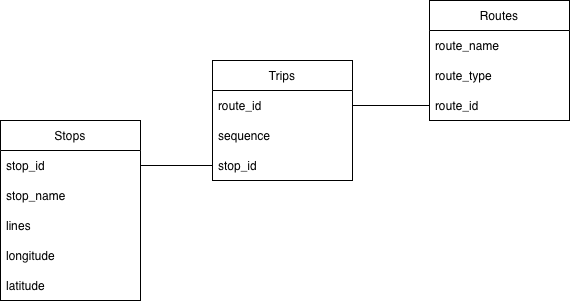
\includegraphics[width=0.7\linewidth]{Immagini/Capitoli/cap1/data_integration.png}
    \caption{Relazioni tra i dataset ridotti}
    \label{fig:data integration}
\end{figure}
\vspace{1em}

La figura \ref{fig:data integration} presenta anche le relazioni esistenti tra i dataset. Ai fini della costruzione del grafo sono stati comunque mantenuti separati, poiché questa scelta agevolava le iterazioni sui dati necessarie alla costruzione del grafo.
\chapter{Grafo PTN}
\label{cap2}

Per analizzare le caratteristiche complesse della PTN, bisogna prima costruire e rappresentare la rete. Il modo migliore per rappresentarla è attraverso un \textbf{grafo}, le cui caratteristiche saranno meglio approfondite nel corso di questo capitolo.

\section{Struttura PTN}
In un approccio generale, si potrebbe voler considerare un modello dinamico della PTN includendo capacità di carico dei convogli e delle linee, numero di passeggeri delle tratte e frequentazione degli itinerari insieme ad una visione completa della struttura PTN, ovvero le caratteristiche \textbf{topologiche} e \textbf{connettive} della rete \cite{vonFerber2012LondonParis}. \\
In assenza dei dati necessari per un simile approccio, questo studio si restringe all'analisi della struttura PTN, con l'obiettivo di studiare le caratteristiche strutturali, per poi analizzare il comportamento, in termini di \textit{resilienza} e \textit{vulnerabilità}, rispetto a determinate condizioni di \textit{stress strutturale}.

\section{Modello PTN}
L'osservazione che i percorsi di una città formino una \textbf{rete} è applicata da secoli, basti pensare all'utilizzo della \textit{teoria dei grafi} per risolvere il \textit{Problema dei ponti di Königsberg}.

\vspace{1em}
\begin{figure}[h!]
    \centering
    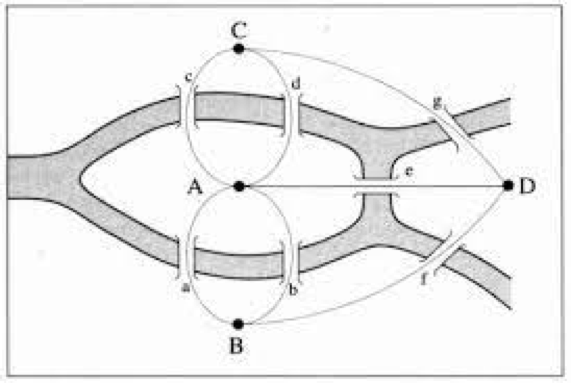
\includegraphics[width=0.4\linewidth]{Immagini//Capitoli//cap2/ponti.png}
    \caption{Grafo del problema dei ponti di Königsberg}
    \label{fig:Rappresentazione a grafo del problema dei ponti di Königsberg}
\end{figure}
\vspace{1em}

Ma che queste reti siano anche \textbf{complesse} è un concetto che si forma in tempi più moderni, con l'aumentare della complessità dei trasporti. Le \textbf{reti complesse} sono diventate recentemente il nucleo di un nuovo campo della conoscenza \cite{vonFerber2012LondonParis} che affonda le proprie radici nella \textit{teoria dei grafi} e nella \textit{statistica}.

\subsection{Modellazione come grafo complesso}
Da un punto di vista puramente matematico, una \textit{rete} non è altro che un \textbf{grafo} $G$ definito da un insieme $V$ di \textit{vertici} e un insieme $E$ di archi che collegano coppie di vertici.

$$
G = (V, E)
$$

Numerose strutture naturali e artificiali possono essere descritte in termini di \textit{grafi}, ma posseggono proprietà differenti da quelli che vengono chiamati \textit{grafi classici}. Tali reti sono classificate come \textbf{reti complesse}. \\
Alcuni esempi sono i sistemi biologici, gli ecosistemi, le reti sociali o le \textit{reti artificiali} come quelle di comunicazione o \textbf{di trasporto}.

Le reti complesse sono strutture \textit{compatte}, a volte definite \textit{piccoli mondi}, con poca distanza tra i nodi, un alto livello di correlazione e auto-organizzazione. Dimostrano resilienza rispetto ad attacchi casuali, d'altra parte hanno dimostrato anche una particolare vulnerabilità rispetto agli attacchi mirati dove con \textit{attacco} si intende la perdita di nodi o archi della rete.

\subsection{Modellazione in L-Space}
Per analizzare le varie proprietà di una PTN si deve iniziare dal modellare correttamente la \textit{topologia} della rete. Due delle modalità più usate sono chiamate $\mathbb{L}$-space e $\mathbb{P}$-space.

\vspace{1em}
\begin{figure}[h!]
  \centering
  % --- Prima immagine (a) ---
  \begin{subfigure}[b]{0.2\textwidth}
    \centering
    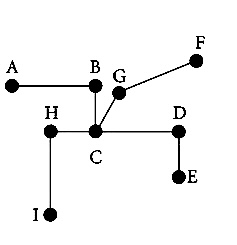
\includegraphics[width=\textwidth]{Immagini/Capitoli/cap2/L-space.jpg}
    \caption{}
    \label{fig:a l-space}
  \end{subfigure}
  \hspace{0.1\textwidth}
  % --- Seconda immagine (b) ---
  \begin{subfigure}[b]{0.3\textwidth}
    \centering
    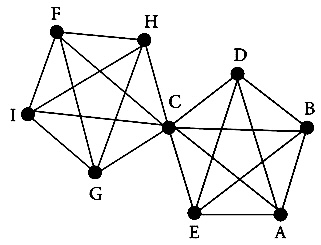
\includegraphics[width=\textwidth]{Immagini/Capitoli/cap2/P-space.jpg}
    \caption{}
    \label{fig:b p-space}
  \end{subfigure}
  % --- Didascalia generale ---
  \caption{Confronto tra una rappresentazione in $\mathbb{L}$-space (a) e $\mathbb{P}$-space (b).}
  \label{fig:confronto L-space P-space}
\end{figure}
\vspace{1em}

In questo studio si è usata la rappresentazione in figura \ref{fig:a l-space} perchè è quella che riproduce più fedelmente la \textit{topologia reale} della PTN. Tale rappresentazione $\mathbb{L}$-space consiste in un insieme di nodi che rappresentano \textit{fermate} e archi che rappresentano un \textit{collegamento} tra due fermate che esiste \textit{se e solo se} sono due fermate consecutive in almeno un \textit{percorso} \cite{vonFerber2012LondonParis}.

Il grado di ogni nodo in questa rappresentazione non è altro che il numero di direzioni \cite{SienkiewiczHolyst2005} che si possono intraprendere dal nodo stesso.

\section{Costruzione del grafo PTN}
Spostandosi su un punto di vista implementativo, il grafo relativo alla PTN in studio è stato costruito con l'ausilio della libreria \textbf{igraph} \cite{igraph} in Python, seguendo la struttura definita in figura \ref{fig:data integration} e costruendo quindi prima i nodi della rete e poi i vari collegamenti, rispettando le relazioni presenti nel dataset dei \textit{Trips}.

\subsection{Costruzione dei nodi}
Per evitare di includere nodi non presenti in alcun percorso, si sono costruiti a partire da una lista univoca dei nodi presenti in \textit{Trips}, acquisendo poi gli attributi dal dataset degli \textit{Stops}. Ogni nodo costruito presenta quindi la seguente struttura:
\begin{itemize}
    \item \texttt{name} id univoco numerico della fermata
    \item \texttt{stop-name} nome della fermata
    \item \texttt{longitude} longitudine della posizione geografica
    \item \texttt{latitude} latitudine della posizione geografica
    \item \texttt{lines} insieme di linee che transitano per la fermata
\end{itemize}

\subsection{Costruzione degli archi}
Per ogni percorso presente in \textit{Routes}, è stata ricostruita la sequenza di nodi appartenenti al percorso con il dataset \textit{trips}. Ogni arco costruito presenta quindi la sequente struttura:
\begin{itemize}
    \item \texttt{edges} coppia di nodi ai vertici dell'arco
    \item \texttt{lines} insieme di linee che transitano sull'arco, nella PTN in studio ogni arco corrisponde ad una sola linea, ma per generalizzare la struttura si è mantenuta comunque la possibilità di assegnare un arco a più linee
\end{itemize}

\subsection{Ridenominazione dei nodi}
Come evidenziato nell'analisi del dataset nella sezione \ref{subsec: analisi del dataset dellef ermate} alcune fermate, quindi alcuni nodi, pur essendo lo stesso nodo sono stati identificati in modi diversi a seconda della linea che servono. Per questa ragione, tali nodi presenti in \ref{tab:Ridenominazione di nodi con doppia identificazione} sono stati fusi in un solo nodo.

\vspace{1em}
\begin{table}[h!]
\centering
\begin{tabular}{lll}
\hline
\textbf{Nuova denominazione} & \textbf{Denominazioni precedenti} \\
\hline
Loreto &  Loreto M2, Loreto M1 \\
Cadorna & Cadorna FN M1, Cadorna FN M2\\
Duomo &  Duomo M1, Duomo M3 \\
Lotto &  Lotto FieraMilanoCity, Lotto M5\\
San Ambrogio &  S.Ambrogio, San Ambrogio \\
\hline
\end{tabular}
\caption{Ridenominazione di nodi con doppia identificazione}
\label{tab:Ridenominazione di nodi con doppia identificazione}
\end{table}
\vspace{1em}
\chapter{Analisi della PTN}
\label{cap3}
Ora che i dataset sono stati convertiti in una rappresentazione a \textit{grafo} e quindi la rete PTN è un grafo è possibile procedere alla sua analisi.

\section{Analisi spaziale del grafo}
Il grafo potrebbe essere semplicemente visualizzato con una delle topologie classiche dei grafi, ma perderebbe, almeno graficamente, la sua struttura \textit{topologica} reale. È utile infatti non solo visualizzare il grafo, ma anche visualizzarlo con le stesse distanze e la stessa distribuzione che i nodi hanno nella realtà da un punto di vista \textbf{geografico} \cite{Candelieri2019}.

\vspace{1em}
\begin{figure}[h!]
    \centering
    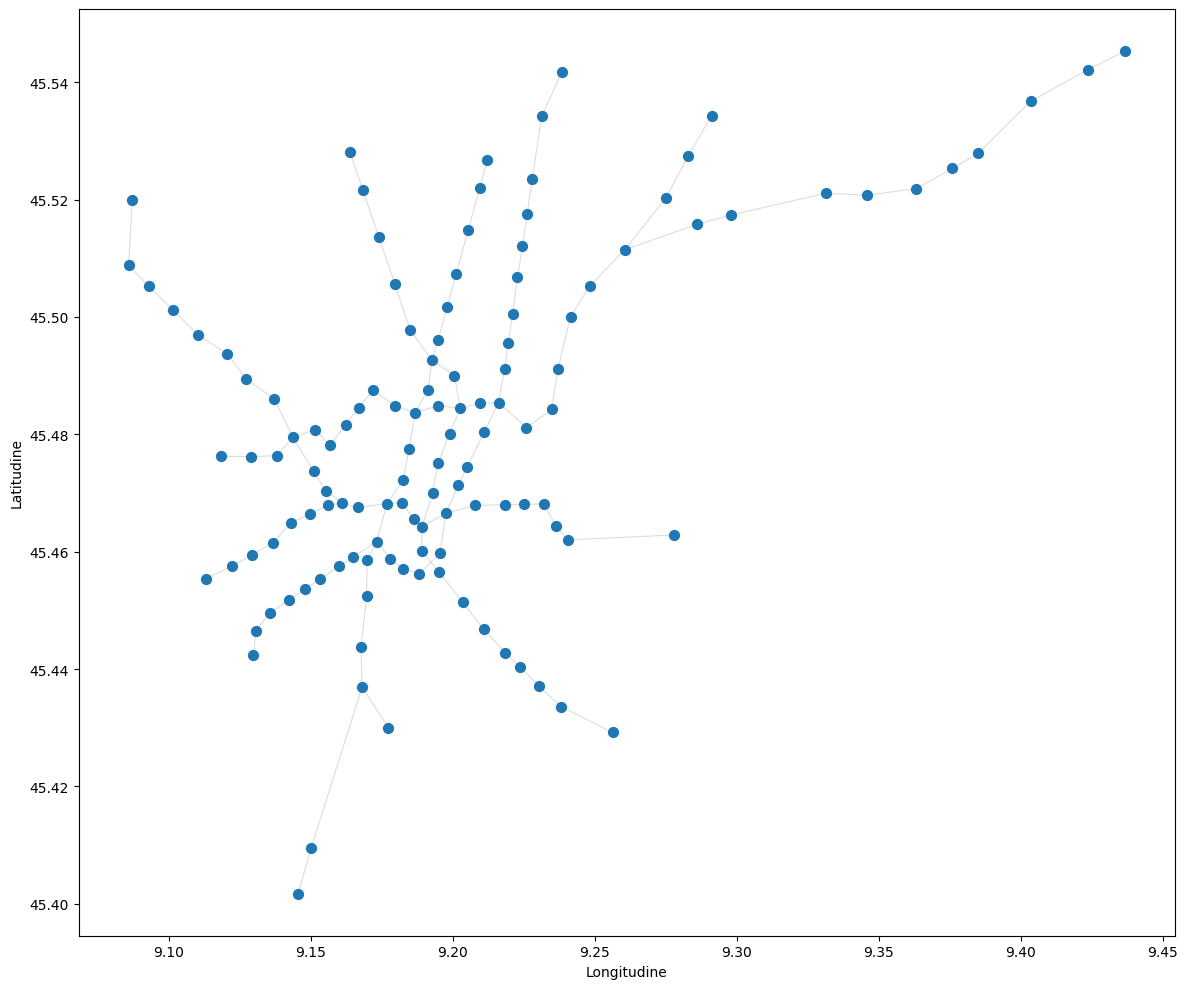
\includegraphics[width=0.8\linewidth]{Immagini//Capitoli//cap3/rete_atm.png}
    \caption{Rete Metropolitana di Milano}
    \label{fig:Rete Metropolitana di Milano}
\end{figure}
\vspace{1em}

Per questa ragione si sono utilizzate le informazioni disponibili di \textbf{latitudine} e \textbf{longitudine} per ottenere la rappresentazione del grafo completo in figura \ref{fig:Rete Metropolitana di Milano}.

\subsection{Analisi spaziale dei sottografi}
Oltre al grafo principale, è possibile visualizzare anche dei \textit{sottografi} corrispondenti alle singole linee metropolitane, discriminando nodi e archi sulla base dell'attributo \texttt{lines} che identifica, appunto, a quale delle linee appartengono.

\vspace{1em}
\begin{figure}[htbp]
  \centering
  % --- Riga 1 ---
  \begin{subfigure}[b]{0.40\textwidth}
    \centering
    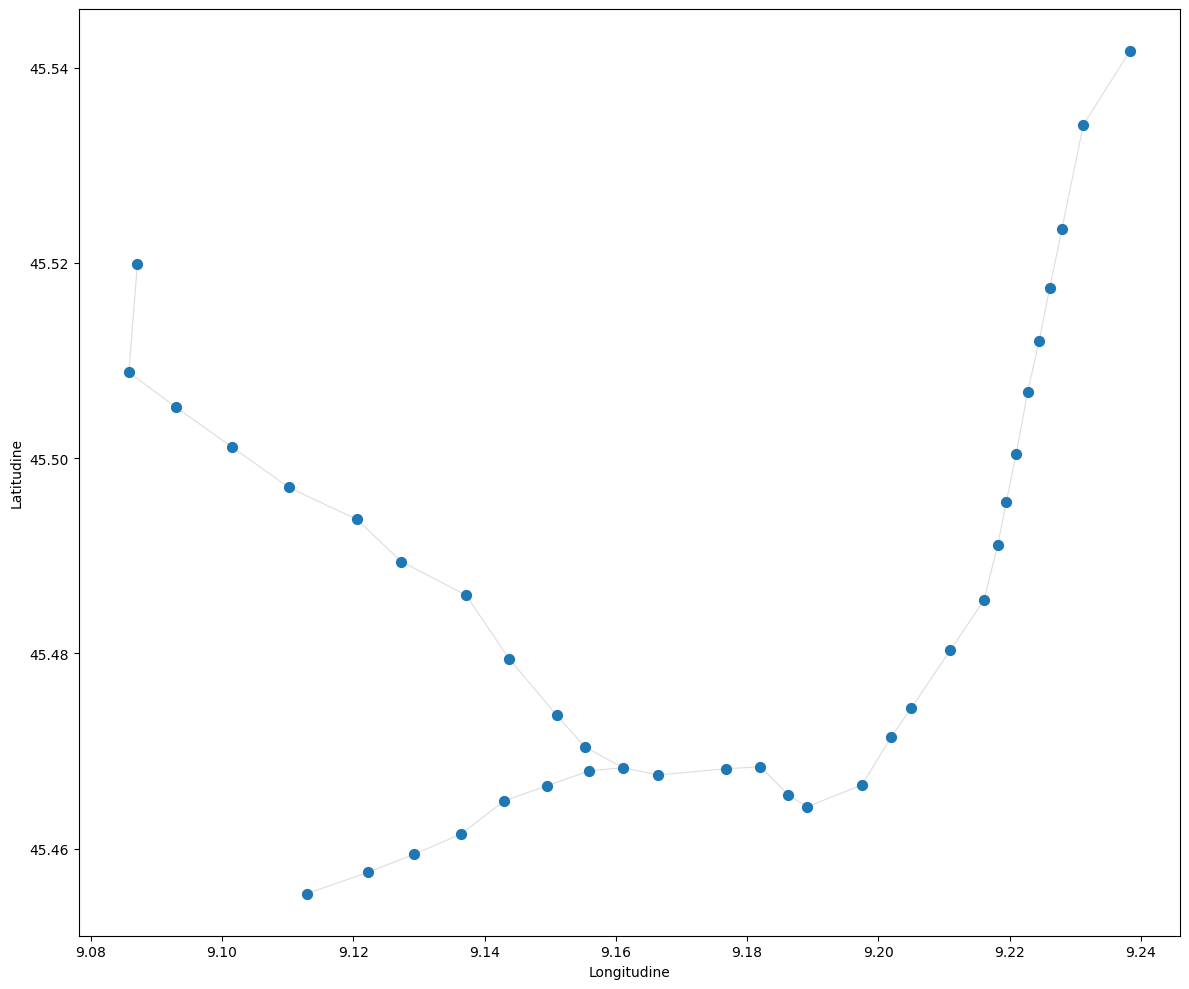
\includegraphics[width=\textwidth]{Immagini/Capitoli/cap3/rete_1.png}
    \caption{Linea 1}
    \label{fig:m1}
  \end{subfigure}%
  \hspace{0.03\textwidth}
  \begin{subfigure}[b]{0.40\textwidth}
    \centering
    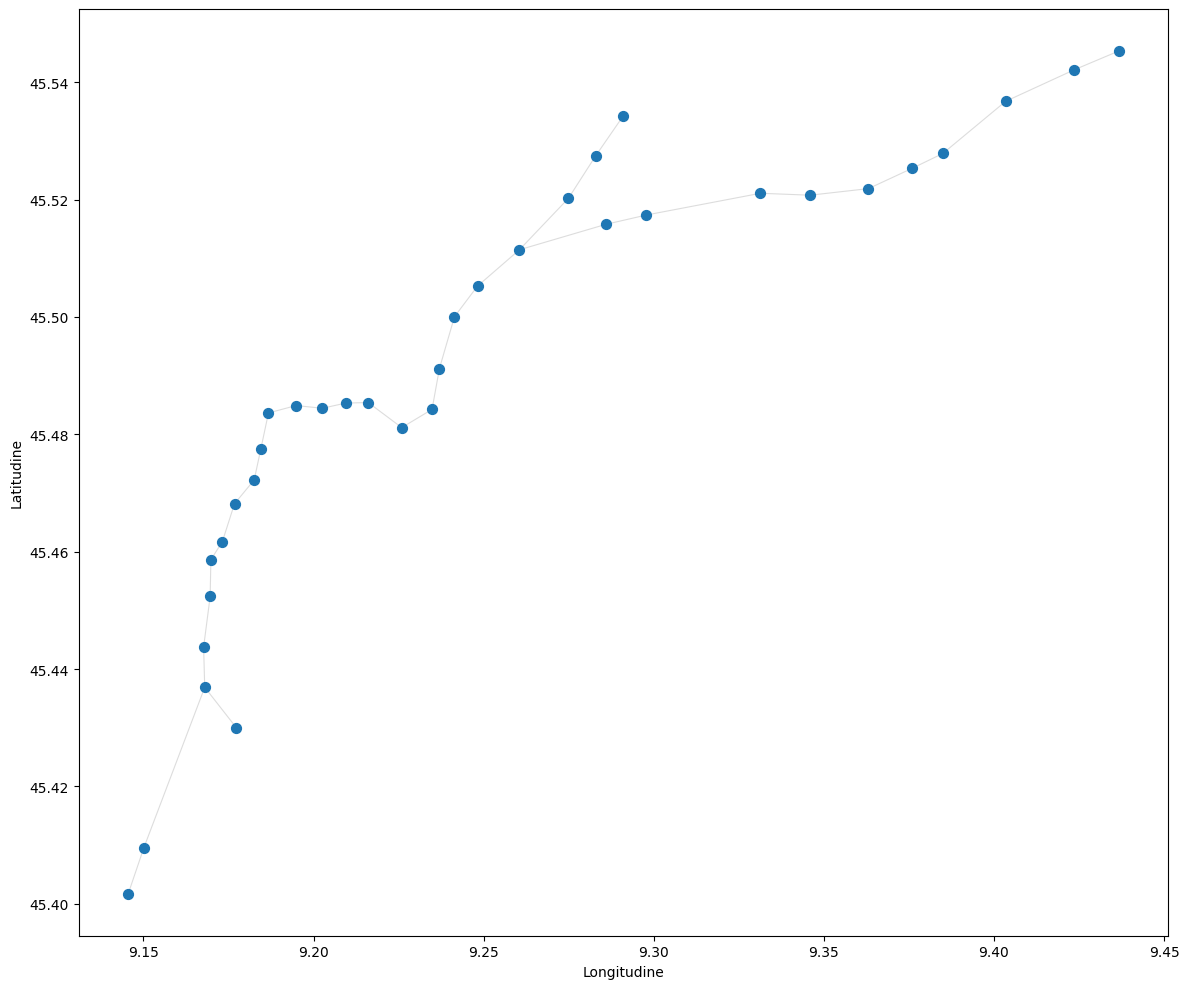
\includegraphics[width=\textwidth]{Immagini/Capitoli/cap3/rete_2.png}
    \caption{Linea 2}
    \label{fig:m2}
  \end{subfigure}

  % --- Riga 2 ---
  \vspace{0.02\textheight}
  \begin{subfigure}[b]{0.40\textwidth}
    \centering
    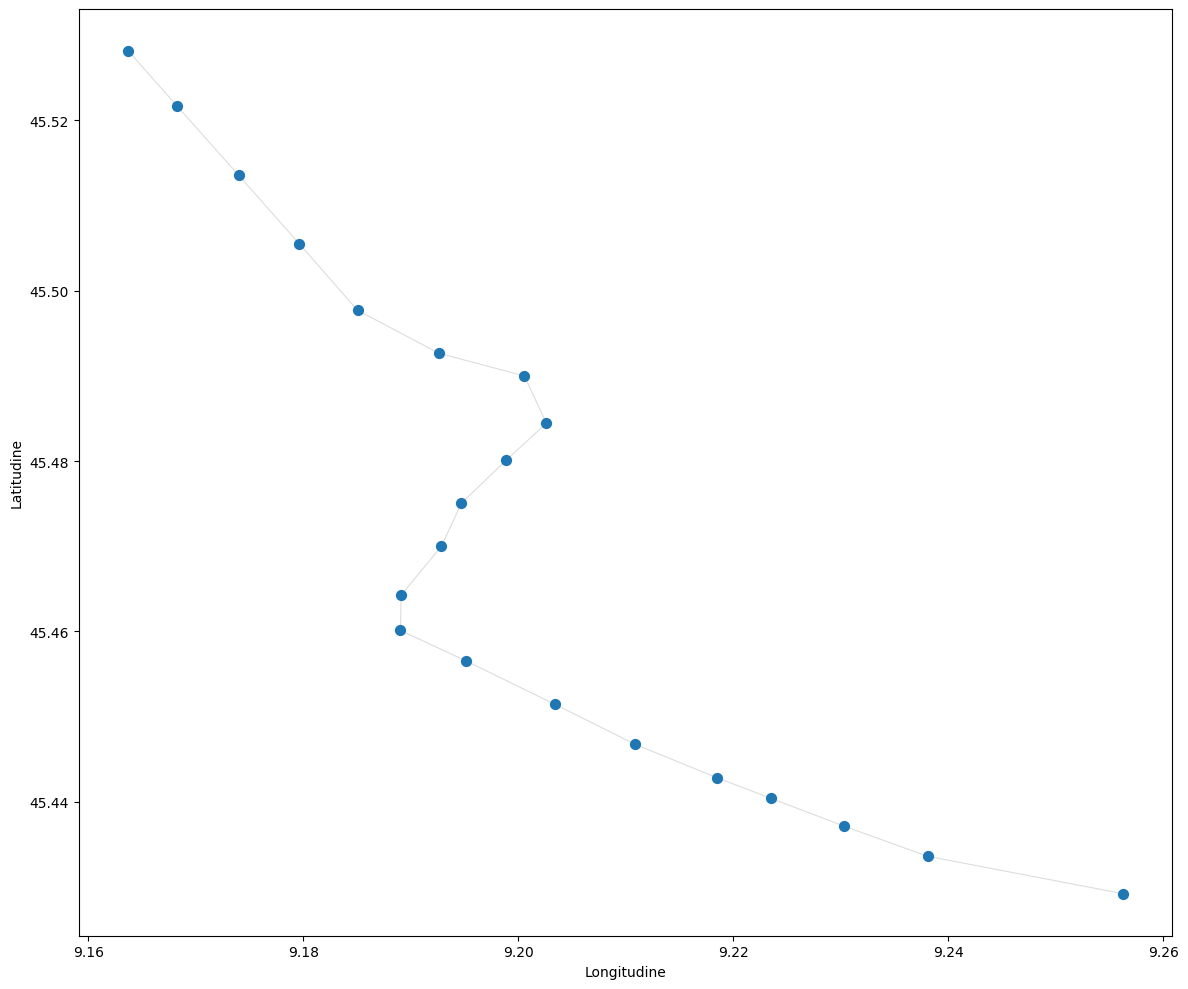
\includegraphics[width=\textwidth]{Immagini/Capitoli/cap3/rete_3.png}
    \caption{Linea 3}
    \label{fig:m3}
  \end{subfigure}%
  \hspace{0.03\textwidth}
  \begin{subfigure}[b]{0.40\textwidth}
    \centering
    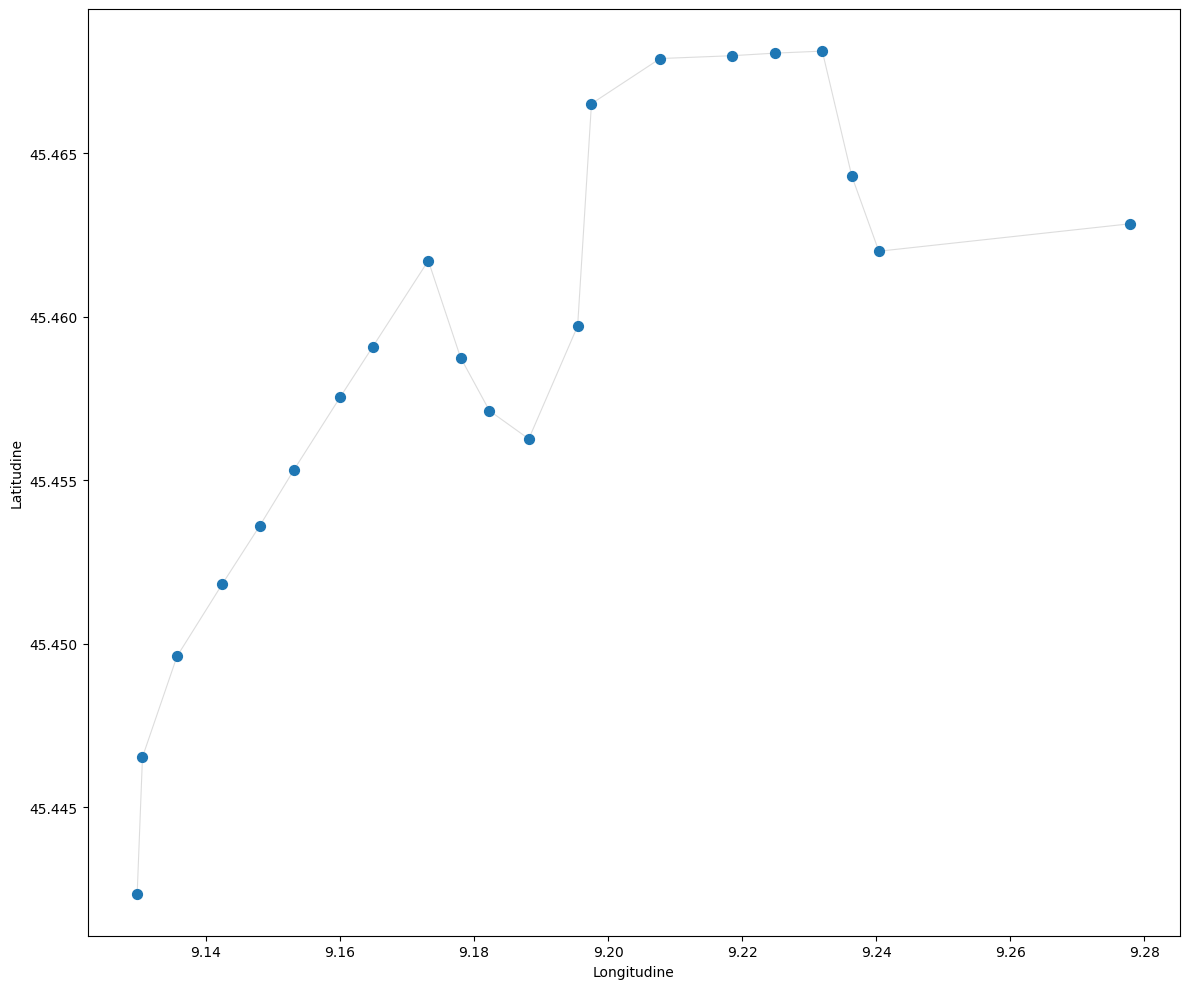
\includegraphics[width=\textwidth]{Immagini/Capitoli/cap3/rete_4.png}
    \caption{Linea 4}
    \label{fig:m4}
  \end{subfigure}

  % --- Riga 3 (centrata) ---
  \vspace{0.02\textheight}
  \begin{subfigure}[b]{0.40\textwidth}
    \centering
    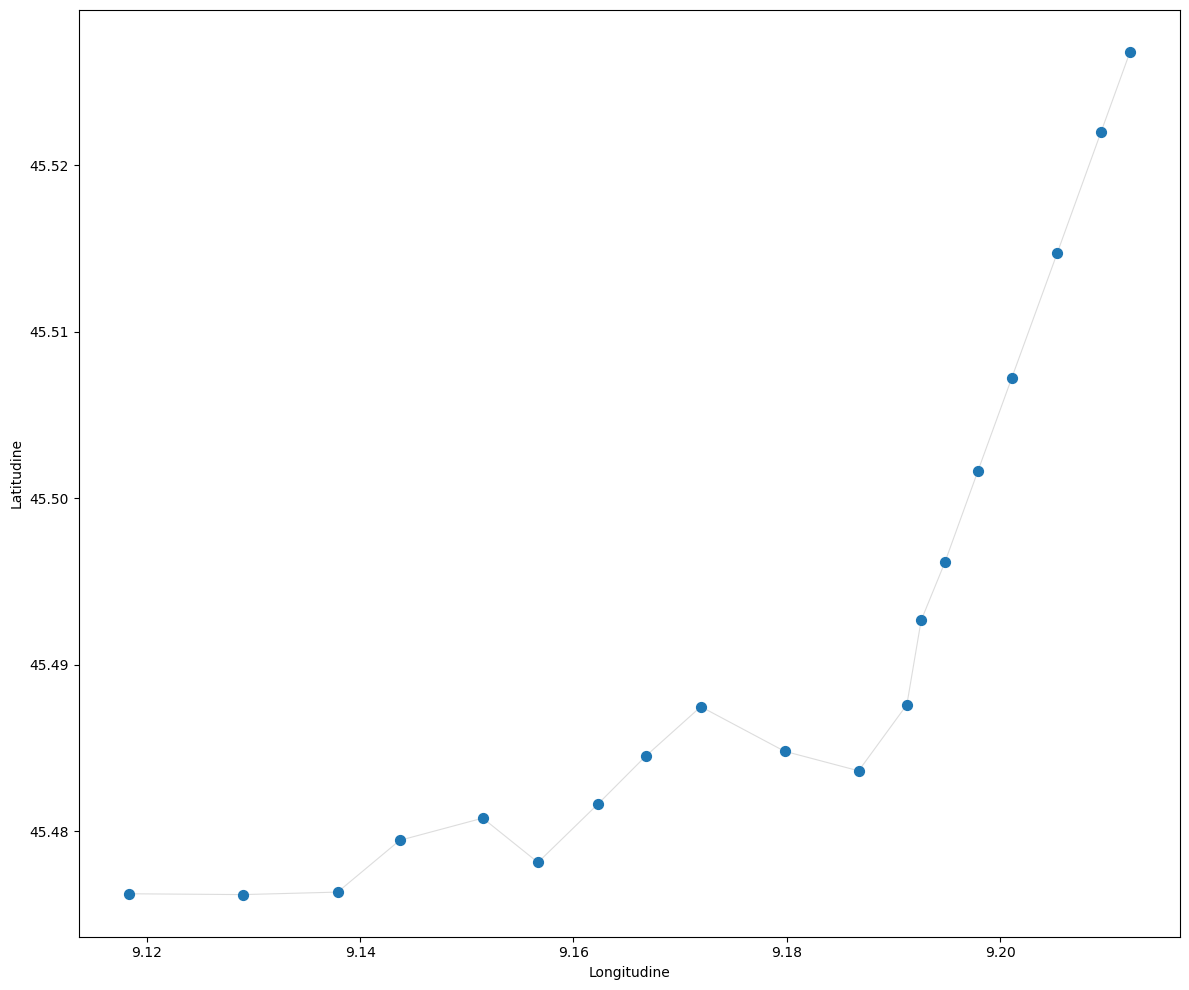
\includegraphics[width=\textwidth]{Immagini/Capitoli/cap3/rete_5.png}
    \caption{Linea 5}
    \label{fig:m5}
  \end{subfigure}

  % --- Didascalia generale ---
  \caption{Sottografi corrispondenti alle linee metropolitane.}
  \label{fig:sottografi}
\end{figure}

\section{Analisi dei nodi e degli archi}
Il grafo si compone di \textbf{125} nodi e \textbf{129} archi. Nella realtà, le stazioni sono 134 se contate singolarmente, ma si ricorda che nel grafo in studio le stazioni con nomenclature diverse ma fisicamente uguali sono state unite in un unico nodo. 

\vspace{1em}
\begin{table}[h!]
\centering
\begin{tabular}{l c c}
\hline
\textbf{Linea} & \textbf{Numero di vertici} & \textbf{Numero di archi} \\
\hline
Linea 1 & 38 & 37\\
Linea 2 & 35 & 34\\
Linea 3 & 21 & 20\\
Linea 4 & 21 & 20\\
Linea 5 & 19 & 18\\
\hline
\end{tabular}
\caption{Numero di vertici e archi per linea}
\label{tab: Numero di vertici e archi per linea}
\end{table}
\vspace{1em}

Nella tabella \ref{tab: Numero di vertici e archi per linea} sono presenti il numero di vertici e archi per ogni linea, in questo caso il numero di vertici corrisponde esattamente al numero di stazioni reali.

\section{Analisi dei gradi}
La rete presenta nodi con gradi che vanno da un minimo di \textbf{1}, ovvero i nodi capolinea, ad un massimo di \textbf{4} per i nodi di interscambio.

\vspace{1em}
\begin{table}[h!]
\centering
\begin{tabular}{l c c}
\hline
\textbf{Grado} & \textbf{Numero di vertici} & \textbf{Distribuzione} \\
\hline
1 & 13 & 10.4\% \\
2 & 100 & 80.0\% \\
3 & 3 & 2.4\% \\
4 & 9 & 7.2\% \\
\hline
\end{tabular}
\caption{Gradi dei nodi della rete}
\label{tab: Gradi dei nodi della rete}
\end{table}
\vspace{1em}

In tabella \ref{tab: Gradi dei nodi della rete} si può già notare che il grado più comune è il \textbf{2}, caratteristica tipica di \textbf{reti prevalentemente lineari} come quelle \textbf{metropolitane}, in cui ci sono diverse linee che si sviluppano radialmente con alcuni \textbf{interscambi} tipicamente situate al centro della rete. Questa caratteristica è fortemente visibile in figura \ref{fig: Distribuzione dei gradi dei nodi}.

\vspace{1em}
\begin{figure}[h!]
    \centering
    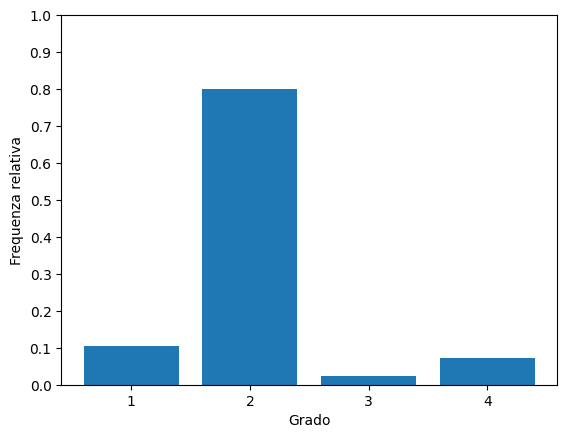
\includegraphics[width=0.5\linewidth]{Immagini//Capitoli//cap3/dist_gradi.png}
    \caption{Distribuzione dei gradi dei nodi}
    \label{fig: Distribuzione dei gradi dei nodi}
\end{figure}
\vspace{1em}

Gli unici nodi con grado \textbf{3} sono quelli di \textbf{diramazione}, caratteristiche delle linee \textit{1} e \textit{2} che si sviluppano in diversi rami, come evidenziato nelle figure \ref{fig:m1} e \ref{fig:m2}.

Da un punto di vista più formale, si ottengono le seguenti metriche:
\[
\begin{array}{cccc}
\hline
k_{\min} & k_{\max} & \langle k \rangle & \sigma_k \\
\hline
1 & 4 & 2.064 & 0.642 \\
\hline
\end{array}
\]

Il grado minimo indica la presenza di nodi terminali \textit{capolinea}, il grado massimo indica invece la presenza di nodi con al più 4 connessioni dirette. La rete non ha quindi degli \textit{hub} con una forte influenza, ma fungono comunque da nodi hub di interscambio.

Il grado medio è molto vicino a 2 e la deviazione standard è piuttosto bassa, confermando la presenza di molti nodi di grado 2.

\subsection{Distribuzione topografica dei gradi}
In figura \ref{fig: Distribuzione topologica dei gradi dei nodi} è rappresentata la distribuzione dei gradi da un punto di vista topografico, con i nodi colorati in base al proprio grado.

\vspace{1em}
\begin{figure}[h!]
    \centering
    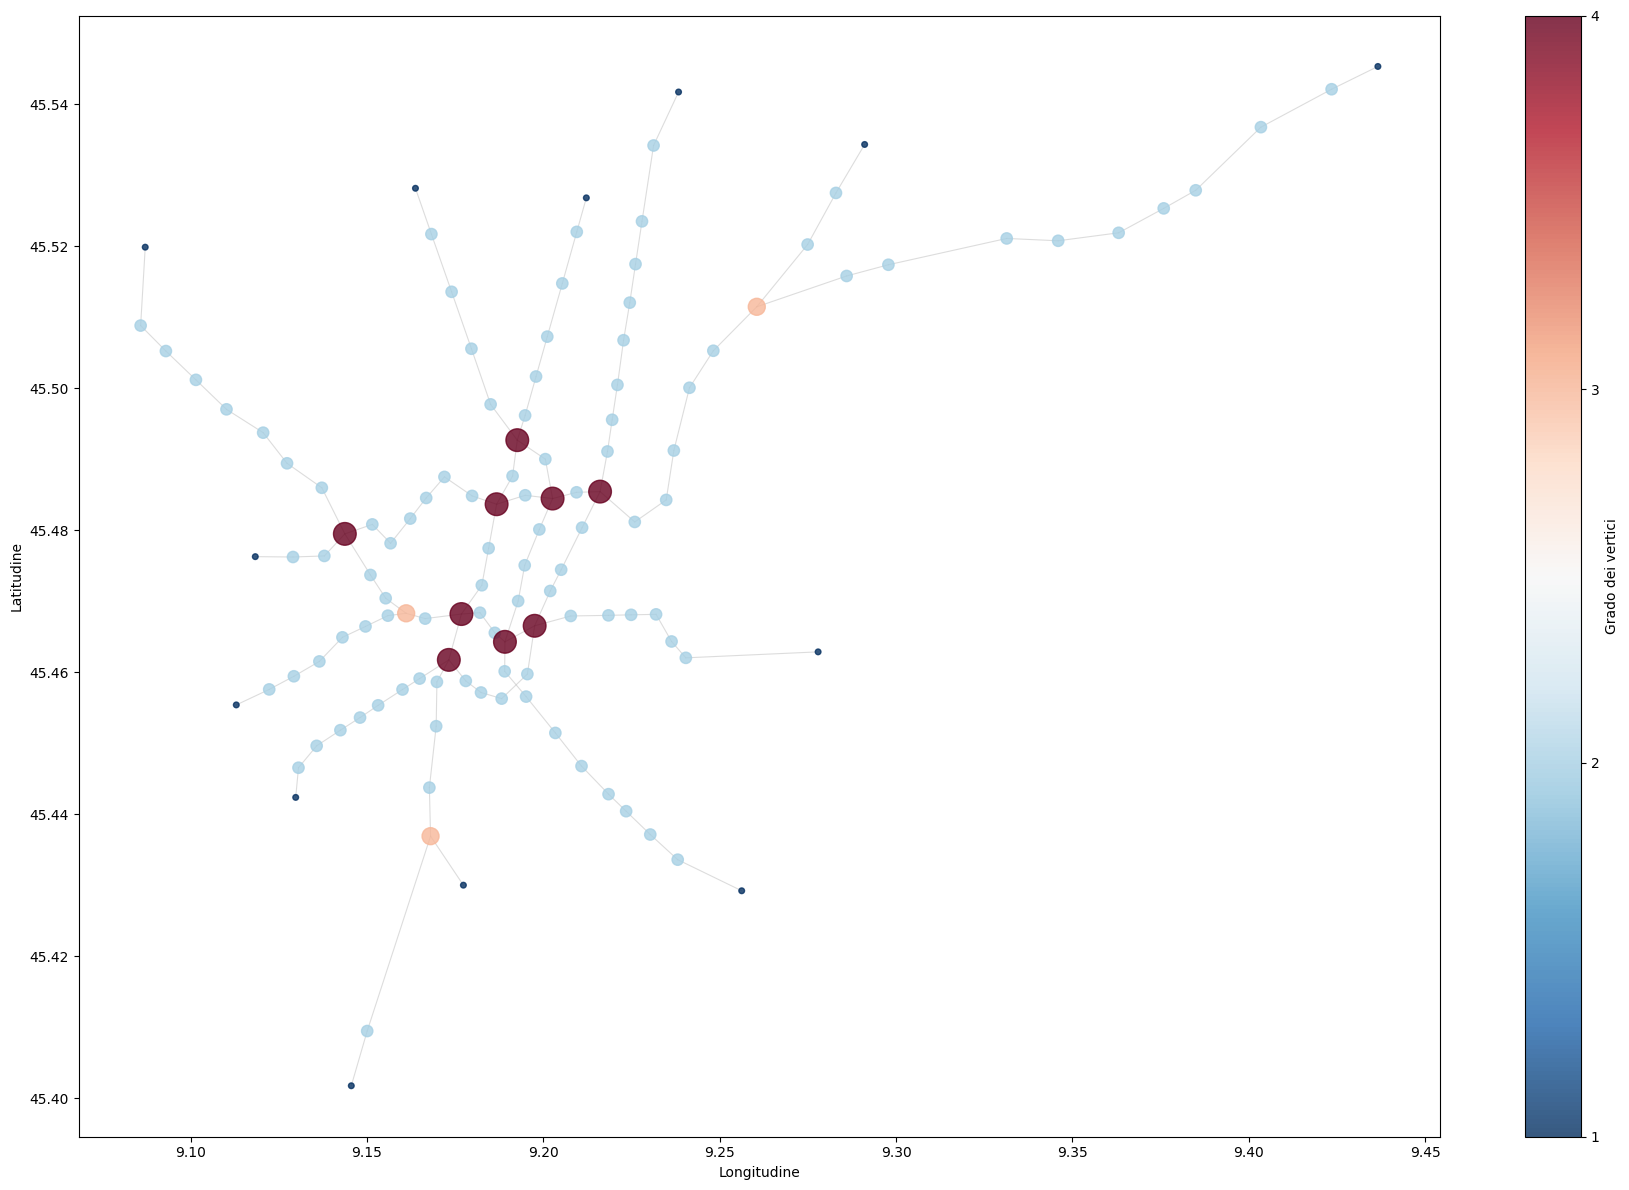
\includegraphics[width=0.8\linewidth]{Immagini//Capitoli//cap3/dist_gradi_mappa.png}
    \caption{Distribuzione topografica dei gradi dei nodi}
    \label{fig: Distribuzione topologica dei gradi dei nodi}
\end{figure}
\vspace{1em}

La rete mostra una configurazione \textit{radiale}, con diversi rami che si diramano dal centro verso la periferia, una struttura tipica delle reti metropolitane. \\
I nodi ad alto grado rappresentano snodi principali, dove convergono più linee, evidenti sono nella figura \ref{fig: Distribuzione topologica dei gradi dei nodi} le stazioni di \textit{Duomo} e \textit{Centrale FS}. I nodi periferici si trovano invece ai margini, coerentemente con il ruolo di \textit{capolinea}.

\section{Analisi dei cammini}
Le metriche principali calcolabili sui cammini sono riassunte di seguito.

\[
\begin{array}{cccc}
\hline
\mathrm{diam}(G) & \ell & E(G) & r(G) \\
\hline
35 & 12.101 & 0.1262 & 18 \\
\hline
\end{array}
\]

\subsection{Distanza massima e minima}
La \textbf{distanza massima} tra due nodi, ovvero il diametro $\mathrm{diam}(G)$ indica che le due stazioni più lontane nella rete sono separate da 35 fermate, il che rappresenta anche l'estensione complessiva della rete.

La \textbf{distanza minima}, ovvero la distanza dal nodo più centrale a quello più lontano chiamato raggio $r(G)$, indica che dal nodo più centrale si può raggiungere qualsiasi altra fermata con un cammino lungo al massimo 18.

\subsection{Distanza media minima}
In figura \ref{fig: Distribuzione dei cammini} sono rappresentate tutte le distanze minime tra coppie di nodi, ovvero di stazioni, della rete. La maggior parte dei nodi ha un cammino compreso tra 10 e 13, la coda destra mostra che esistono comunque coppie di nodi maggiormente distanti.


\vspace{1em}
\begin{figure}[h!]
    \centering
    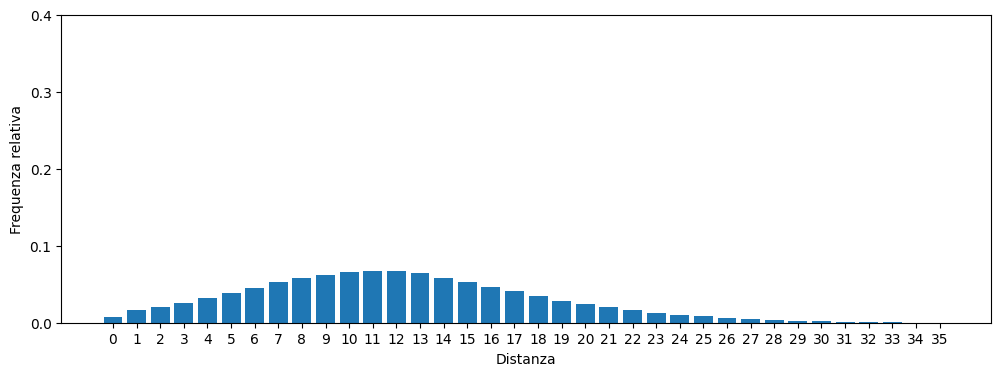
\includegraphics[width=0.8\linewidth]{Immagini//Capitoli//cap3/dist_cammini.png}
    \caption{Distribuzione dei cammini}
    \label{fig: Distribuzione dei cammini}
\end{figure}
\vspace{1em}

Quanto evidenziato in figura \ref{fig: Distribuzione dei cammini} si ritrova anche nella \textbf{lunghezza media dei cammini} $\ell$ di valore 12.101, coerente con il picco tra 10 e 13 del grafo.

\subsection{Efficienza globale}
L'efficienza globale $E(G)$ misura quanto efficacemente le informazioni, nel caso in studio i \textit{passeggeri}, possono muoversi attraverso la rete. Il valore di $0.13 \approx 0.1\text{--}0.3$ è tipico di infrastrutture \textbf{geografiche}, in cui i collegamenti devono seguire vincoli fisici e urbanistici.

\section{Analisi strutturale}

\subsection{Componenti connesse}
Essendo una PTN in cui ogni linea si interseca con \textit{almeno un'altra} linea, la \textbf{componente connessa} è \textit{una}, ciò implica che la \textbf{giant component} corrisponde a tutta la rete.

\subsection{Clustering}
Una PTN metropolitana difficilmente presenta stazioni che godono della proprietà di \textit{transitività}, in linea con questa intuizione teorica nella PTN in studio il coefficiente di \textbf{clustering} è pari a \textit{zero}.

\subsection{Assortatività}
Con un \textbf{grado di Assortatività} di -0.0264, la rete è \textbf{disassortativa}, ovvero le stazioni molto connesse tendono a collegarsi a stazioni meno connesse, un comportamento tipico delle reti di trasporto in cui sono presenti \textit{hub} di \textit{modesta entità}, riportati in tabella \ref{tab: Hub score delle stazioni principali}, in uno struttura gerarchica fino ai nodi periferici.

\vspace{1em}
\begin{table}[h!]
\centering
\begin{tabular}{l c}
\hline
\textbf{Stazione} & \textbf{Hub Score} \\
\hline
Centrale FS & 1.000\\
Garibaldi FS & 0.967\\
Cadorna & 0.957\\
Zara & 0.850\\
Duomo & 0.829\\
\hline
\end{tabular}
\caption{Hub score delle stazioni principali}
\label{tab: Hub score delle stazioni principali}
\end{table}
\vspace{1em}

Quindi la rete è efficientemente organizzata per distribuzione del traffico, ma non molto robusta rispetto a guasti negli hub principali, aspetto che sarà \textbf{determinante} nello studio di vulnerabilità della rete nel capitolo \ref{cap5}.


\chapter{Analisi di centralità}
\label{cap4}
Dopo aver descritto le principali caratteristiche strutturali e topologiche della rete metropolitana milanese, è possibile approfondire lo studio del grafo analizzandone le misure di \textbf{centralità}. \\
Queste metriche consentono di valutare l’importanza relativa dei nodi all’interno della rete, non solo in termini di numero di connessioni, ma anche di posizione strategica e di ruolo funzionale nella connettività complessiva del sistema.

\section{Centralità di grado}
La \textbf{degree centrality} indica quanti collegamente diretti o \textit{adiacenze} ha ciascun nodo della rete. Nella figura \ref{fig: Degree Centrality} è rappresentata la distribuzione di questa misurazione.

\vspace{1em}
\begin{figure}[h!]
    \centering
    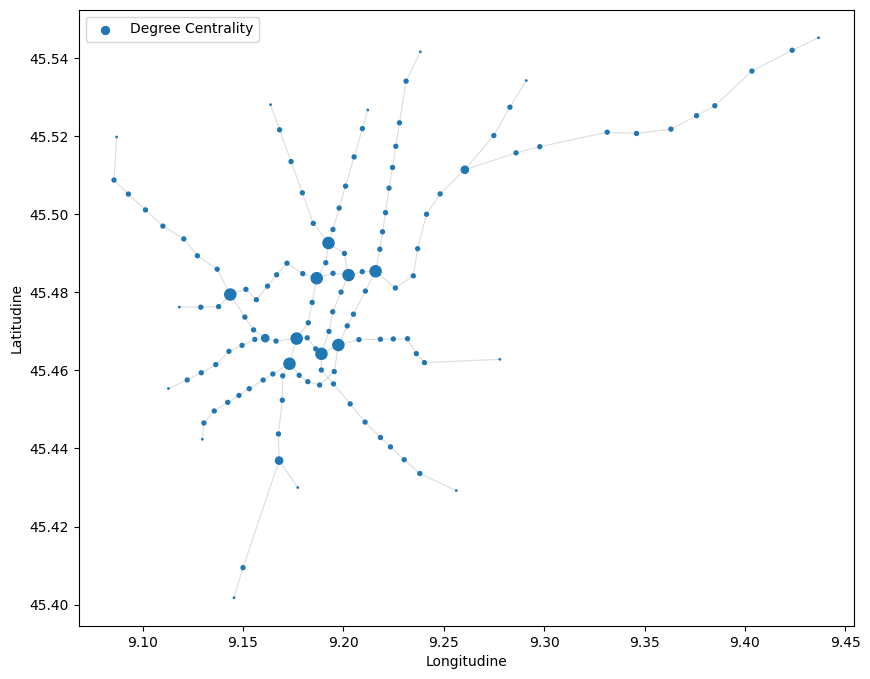
\includegraphics[width=0.8\linewidth]{Immagini//Capitoli//cap4/degree_centr.png}
    \caption{Degree centrality}
    \label{fig: Degree Centrality}
\end{figure}
\vspace{1em}

Valgono tutte le considerazioni sui gradi già affrontante nel corso del capitolo \ref{cap3}.


\section{Centralità di intermediazione}
La \textbf{betweeness centrality} misura quante volte un nodo si trova in un \textit{percorso minimo} tra altre coppie di nodi, ovvero identifica i nodi più rilevanti come quelli che fanno da ponte tra due gruppi di nodi.

\vspace{1em}
\begin{figure}[h!]
    \centering
    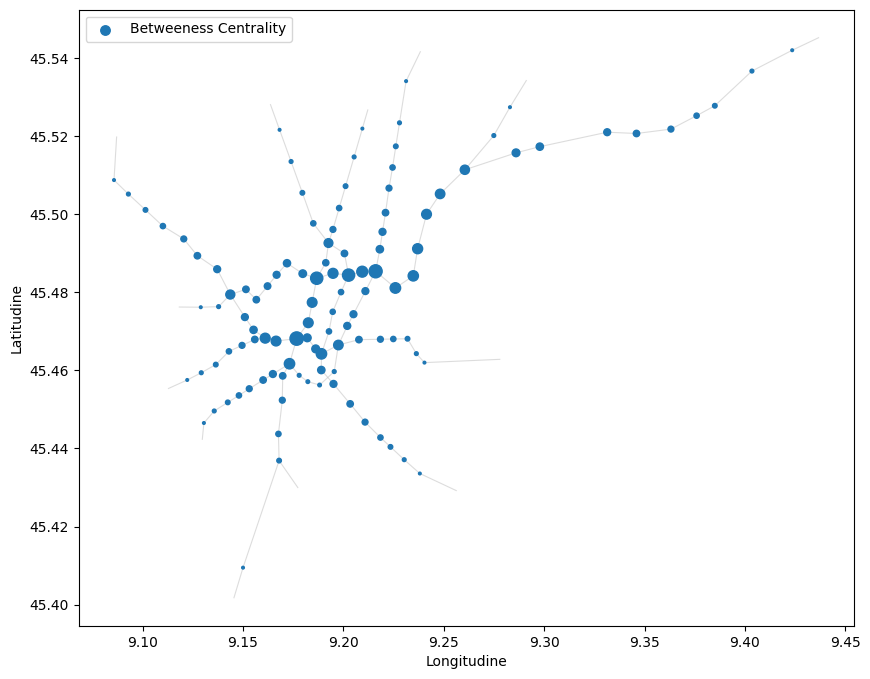
\includegraphics[width=0.8\linewidth]{Immagini//Capitoli//cap4/betw_centr.png}
    \caption{Betweeness centrality}
    \label{fig: Betweeness Centrality}
\end{figure}
\vspace{1em}

In figura \ref{fig: Betweeness Centrality} è rappresentata la distribuzione di questa misurazione, si osserva che i nodi centrali e quelli precedenti a delle diramazioni hanno un'importanza maggiore rispetto ai nodi presenti su diramazioni periferiche.

\subsection{Nodi centrali di intermediazione}
Come ci si potrebbe aspettare, i nodi centrali secondo questa misurazione sono \textit{principalmente} quelli di interscambio, ma ci sono comunque alcuni nodi che, nonostante non siano di interscambio, hanno un alto potere di intermediazione, infatti verificando i primi dieci nodi per centralità di intermediazione:

\begin{center}
CADORNA \\
LORETO \\
GARIBALDI FS \\
CENTRALE FS \\
CAIAZZO \\
PIOLA \\
DUOMO \\
SAN AMBROGIO \\
LAMBRATE FS \\
UDINE \\
\end{center}

si ritrova \textit{ad esempio} la stazione di \textit{PIOLA} prima di quella di \textit{DUOMO}, come alcune stazioni \textit{non} geograficamente centrali come \textit{LAMBRATE FS} e \textit{UDINE}.

\section{Centralità di prossimità}
La \textbf{closeness centality} misura quanto un nodo è vicino, in termini di distanza nel grafo, da tutti gli altri nodi.

\vspace{1em}
\begin{figure}[h!]
    \centering
    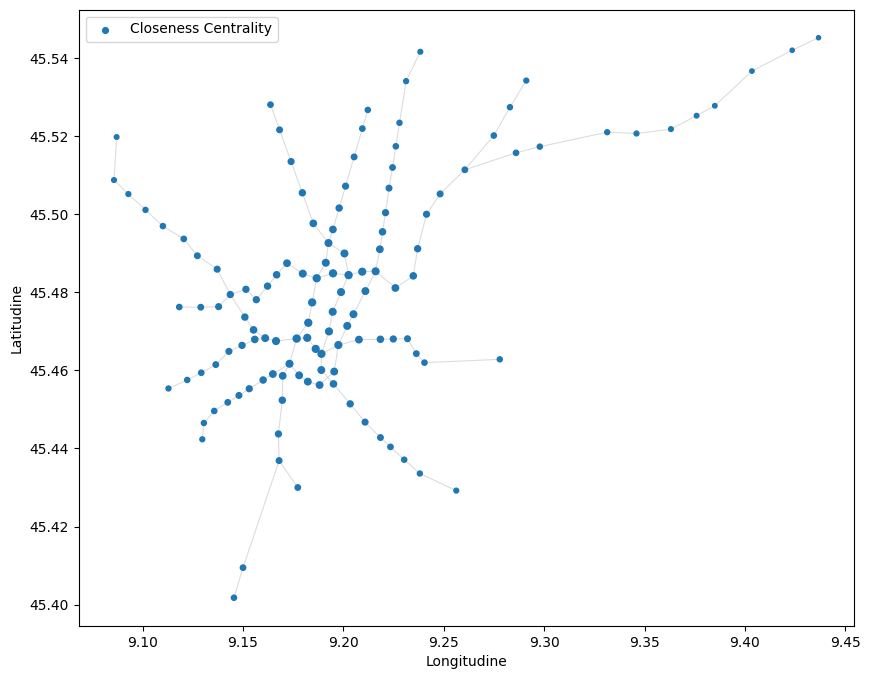
\includegraphics[width=0.8\linewidth]{Immagini//Capitoli//cap4/close_centr.png}
    \caption{Closeness centrality}
    \label{fig: Closeness Centrality}
\end{figure}
\vspace{1em}

In figura \ref{fig: Closeness Centrality} è rappresentata la distribuzione di questa misurazione.

\subsection{Nodi centrali di prossimità}
Anche in questo caso, i nodi più centrali sono quelli che sono anche \textit{geograficamente} più centrali. Più interessante per questa misurazione è invece capire quali nodi sono meno centrali, che intuitivamente dovrebbero essere quelli agli estremi delle diramazioni più lontane dal centro, ovvero la diramazione per \textit{RHO FIERAMILANO} della linea 1 e la diramazione per \textit{GESSATE} della linea 2. In effetti, gli ultimi 8 nodi per centralità di prossimità sono:

\begin{center}
GESSATE \\
CASCINA ANTONIETTA \\
GORGONZOLA \\
VILLA POMPEA \\
BUSSERO \\
RHO FIERAMILANO \\
CASSINA DE PECCHI \\
PERO \\
\end{center}

che sono, a conferma di quanto ipotizzato, proprio stazioni appartenenti alle diramazioni precedentemente evidenziate.

\section{Centralità di autovettore}
La \textbf{eigenvector centrality} valuta l'importanza di un nodo in funzione dell'importanza dei suoi vicini, ovvero un nodo è importante se collegato ad altri nodi importanti.

\vspace{1em}
\begin{figure}[h!]
    \centering
    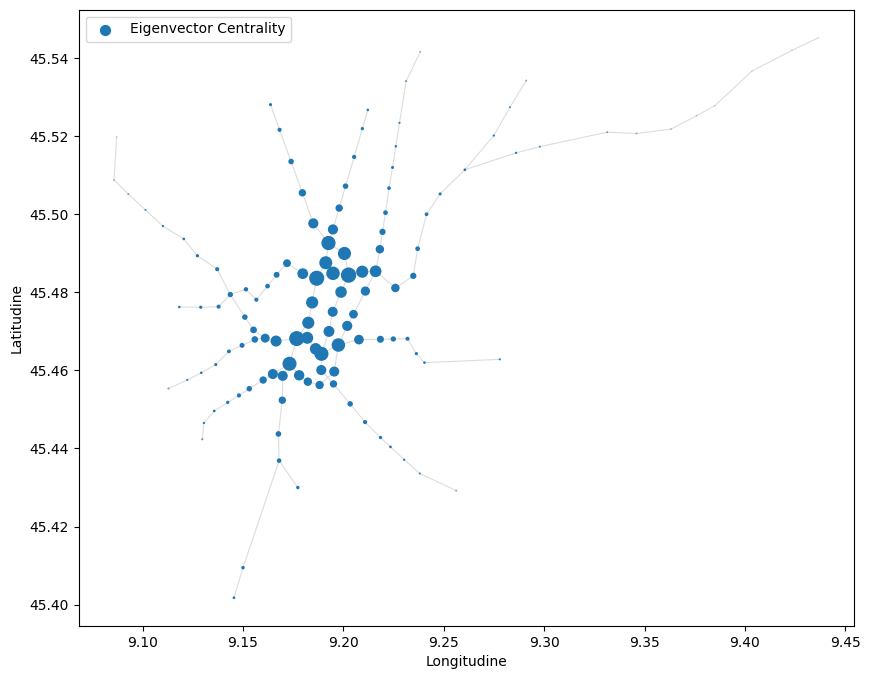
\includegraphics[width=0.8\linewidth]{Immagini//Capitoli//cap4/eigen_centr.png}
    \caption{Eigenvector centrality}
    \label{fig: Eigenvector Centrality}
\end{figure}
\vspace{1em}

In figura \ref{fig: Eigenvector Centrality} è rappresentata la distribuzione di questa misurazione, in cui è maggiormente evidente, rispetto alle altre misure di centralità, quanto i nodi corrispondenti a stazioni \textit{geograficamente} più centrali siamo più importanti rispetto ai nodi periferici, che in questa misurazione diventano del tutto trascurabili e anche difficilmente leggibili in figura.
\chapter{Studio di vulnerabilità}
\label{cap5}

Il concetto di \textbf{vulnerabilità} in una rete complessa mira a \textit{quantificare} la sua \textit{sicurezza} e la sua \textit{stabilità} sotto gli effetti di un qualsiasi tipo di \textit{disfunzione} \cite{MattssonJenelius2015}.

Nelle PTN la vulnerabilità è legata alla \textit{sensibilità alle interruzioni}, in particolare una definizione consolidata e diffusa è la seguente: "\textit{La vulnerabilità in un sistema di trasporto è la suscettibilità ad incidenti che possono portare ad una considerevole riduzione della funzionalità della rete stessa}" \cite{Berdica2002}. 

\section{vulnerabilità in una PTN}
Per studiare la vulnerabilità, bisogna prima comprendere cosa si intende con \textit{attaccare} una rete. \\
Un \textbf{attacco} in una rete è la rimozione intenzionale di nodi o archi con l’obiettivo di ridurre la funzionalità o connettività del sistema \cite{vonFerber2012LondonParis}, può essere eseguito secondo due approcci:
\begin{itemize}
    \item \textbf{Statico} in questo approccio non si considerano gli effetti della rimozione di un nodo, ovvero si assume che, eliminando un nodo, il resto della rete sia comunque operativa;
    \item \textbf{A cascata} in questo approccio, più realistico, si considerano gli effetti della rimozione di un nodo, ovvero si rimuovono i nodi non seguendo l'ordine di rimozione stabilito inizialmente, ma ricalcoldando ogni volta la metrica di riferimento.
\end{itemize}

\subsection{Ordine di attacco}
Nell'analisi di vulnerabilità l'obiettivo è portare la rete allo stremo per studiarne il comportamento in situazioni di gravità crescente, quindi non si rimuove un solo nodo, ma una \textit{successione di nodi} secondo un determinato criterio. Il criterio prescelto discrimina l'attacco in due tipologie:
\begin{itemize}
    \item \textbf{Attacco mirato} si rimuovono progressivamente dei nodi selezionati per importanza, nel caso in studio si effettuerà un attacco mirato per \textit{grado} e uno per \textit{betweenness};
    \item \textbf{Attacco casuale} si rimuovono progressivamente e casualmente dei nodi.
\end{itemize}

\subsection{Criterio di integrità}
Una volta stabilito cosa si intende con \textit{attacco}, bisogna comprendere come \textit{quantificare} gli effetti dell'attacco, ovvero comprendere quanto la rete è \textbf{integra}. \\
Il \textbf{criterio di integrità} più utilizzato \cite{vonFerber2012LondonParis} passa per il concetto di \textbf{componente connessa}: gli effetti di un attacco si comprendono analizzando come varia, in termini di quantità di nodi, la più grande componente connessa della rete.

Si introduce quindi la \textbf{GCC fraction}, che indica la percentuale di nodi della rete facente parte della più grande componente connessa:

$$
    \texttt{GCC fraction} = \frac{\texttt{GCC nodes} }{N}
$$

Questa metrica indica quanto del sistema continua a funzionare: quando la GCC \textbf{collassa}, significa che la rete ha perso la capacità di trasmettere traffico in modo globale.

\section{Aspettative rispetto alle analisi precedenti}
Prima di procedere con uno studio di vulnerabilità puntuale e corretto secondo la letteratura, si possono utilizzare le analisi svolte fino ad ora nei capitoli \ref{cap3} e \ref{cap4} per avere un'aspettativa di quelli che potrebbero essere i risultati successivi.

\subsection{Aspettative dell'attacco casuale}
Le metriche calcolate e le analisi svolte hanno evidenziato la presenza di una \textit{rete lineare}, con una prevalenza di nodi di grado 2. La probabilità che in un attacco casuale venga attaccato un nodo di grado 2 è quindi elevata. Attaccare nodi di questo tipo non comporta una grande vulnerabilità per la rete, perchè i nodi con grado maggiore garantiscono una certa coesione della rete rimanente. 

L'aspettativa è quindi che la rete possa essere meno vulnerabile ad un attacco di questo tipo rispetto che ad un attacco mirato.

\subsection{Aspettative dell'attacco mirato}
Le metriche calcolate e le analisi svolte hanno evidenziato la presenza di alcuni \textit{hub} di piccola dimensione al centro geografico della rete, in cui si concentrano gli \textit{interscambi} tra le linee. 

La dimensione degli hub non giustifica una grande importanza rispetto al resto della rete, ma sono comunque più strategici dei nodi alle diramazioni della rete e quindi l'aspettativa è che un attacco mirato a questi nodi, che sono i primi ad essere attaccati sia per \textit{grado} che per \textit{betweenness}, possa portare ad un \textbf{degrado} \textbf{maggiore} e \textbf{più rapido} della rete rispetto all'attacco casuale. 

\section{Analisi degli attacchi di vulnerabilità}
L'analisi svolta ha considerato 5 situazioni differenti di attacco, riassunte in tabella \ref{tab: Attacchi di vulnerabilità considerati}. Ogni attacco ha operato a partire da una frazione di 0 \textit{nodi rimossi} fino ad un \textbf{massimo} del 50\% di \textit{nodi rimossi}.

\vspace{1em}
\begin{table}[!ht]
\centering
\begin{tabular}{l l l}
\hline
\textbf{Attacco} & \textbf{Tipologia} & \textbf{Note implementative} \\
\hline
Grado & Mirato & In ordine di grado \\
Betweenness & A Cascata & Ricalcolo della betweenness ad ogni iterazione \\
Grado & A Cascata & Ricalcolo della betweenness ad ogni iterazione \\
Betweenness & Mirato & In ordine di betweenness \\
Casuale & Mirato & Media di 12 attacchi indipendenti \\
\hline
\end{tabular}
\caption{Attacchi di vulnerabilità considerati}
\label{tab: Attacchi di vulnerabilità considerati}
\end{table}
\vspace{1em}

L'attacco casuale, per avere una stima più puntuale, è stato svolto diverse volte su diversi ordini casuali dei nodi attaccati. Pertanto, i risultati di questo attacco sono le medie dei risultati dei singoli attacchi casuali.

\subsection{Analisi dell'attacco casuale}
In figura \ref{fig: Attacco di vulnerabilità casuale} è possibile visualizzare la \textit{GCC fraction} in relazione ai \textit{nodi rimossi} negli attacchi casuali. La linea rappresenta la media degli attacchi e l'ombra la deviazione standard.

\vspace{1em}
\begin{figure}[h!]
    \centering
    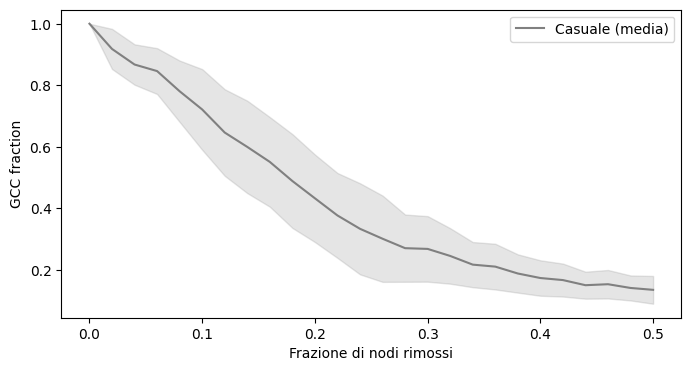
\includegraphics[width=0.8\linewidth]{Immagini//Capitoli//cap5/atk_random.png}
    \caption{Attacco di vulnerabilità casuale}
    \label{fig: Attacco di vulnerabilità casuale}
\end{figure}
\vspace{1em}

Il comportamento medio indica che il \textit{decadimento} è \textbf{graduale}, quasi \textbf{lineare}, serve rimuovere più del 20\% dei nodi per ridurre il GCC sotto il 50\%.

L'intervallo di confidenza resta relativamente ristretto ed evidenzia un comportamento stabile tra le simulazioni.

\subsection{Analisi dell'attacco per grado}
In figura \ref{fig: Confronto attacco di vulnerabilità per grado e per grado a cascata} è possibile visualizzare la \textit{GCC fraction} in relazione ai \textit{nodi rimossi} negli attacchi per grado, in un confronto tra un attacco mirato per grado e in un attacco a cascata per grado.

\vspace{1em}
\begin{figure}[ht!]
    \centering
    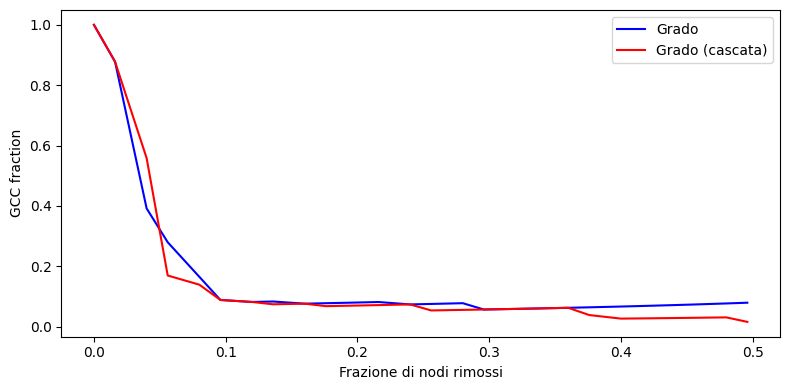
\includegraphics[width=0.8\linewidth]{Immagini//Capitoli//cap5/atk_degree_cfr.png}
    \caption{Confronto attacco di vulnerabilità per grado e per grado a cascata}
    \label{fig: Confronto attacco di vulnerabilità per grado e per grado a cascata}
\end{figure}
\vspace{1em}

Entrambe le curve \textbf{crollano} velocemente, la frazione del GCC scende sotto il 20\% già al 10\% dei nodi rimossi. \\
L'attacco a cascata è leggermente più \textbf{aggressivo}, soprattutto nella discesa iniziale.

Dopo il 15\% di nodi rimossi, entrambe le curve si appiattiscono, indicando un collasso quasi totale della rete.

\subsection{Analisi dell'attacco per betweenness}
In figura \ref{fig: Confronto attacco di vulnerabilità per betweenness e per betweenness a cascata} è possibile visualizzare la \textit{GCC fraction} in relazione ai \textit{nodi rimossi} negli attacchi per betweenness, in un confronto tra un attacco mirato per betweenness e in un attacco a cascata per betweenness.

\vspace{1em}
\begin{figure}[h!]
    \centering
    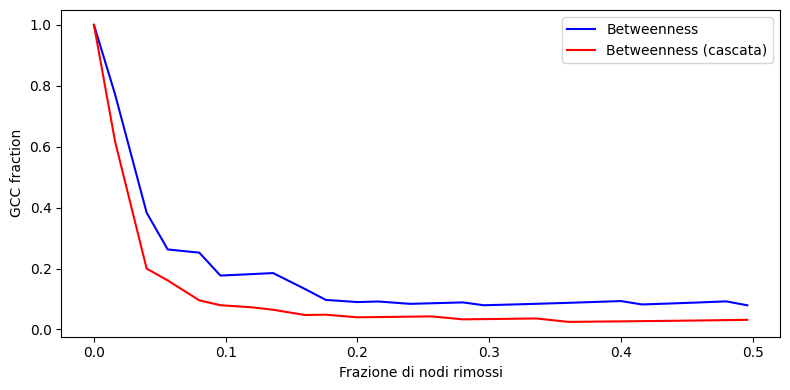
\includegraphics[width=0.8\linewidth]{Immagini//Capitoli//cap5/atk_btw_cfr.png}
    \caption{Confronto attacco di vulnerabilità per betweenness e per betweenness a cascata}
    \label{fig: Confronto attacco di vulnerabilità per betweenness e per betweenness a cascata}
\end{figure}
\vspace{1em}

Analogamente all'attacco precedente, entrambe le curve mostrano un \textbf{crollo} veloce, con una distruzione più repentina da parte dell'attacco \textit{a cascata}: dopo il 10\% dei nodi rimossi la rete è già quasi completamente frammentata.

La rete è dipendente da nodi con elevata betweenness, che fungono da intersezioni tra linee, e l’effetto cascata amplifica questa vulnerabilità: rimuovendo un nodo importante, altri ereditano la caratteristica e vengono rapidamente eliminati.

\subsection{Analisi comparativa degli attacchi}
In figura \ref{fig: Confronto attacchi di vulnerabilità} è possibile visualizzare la \textit{GCC fraction} in relazione ai \textit{nodi rimossi} in confronto a tutti gli attacchi eseguiti.

\vspace{1em}
\begin{figure}[h!]
    \centering
    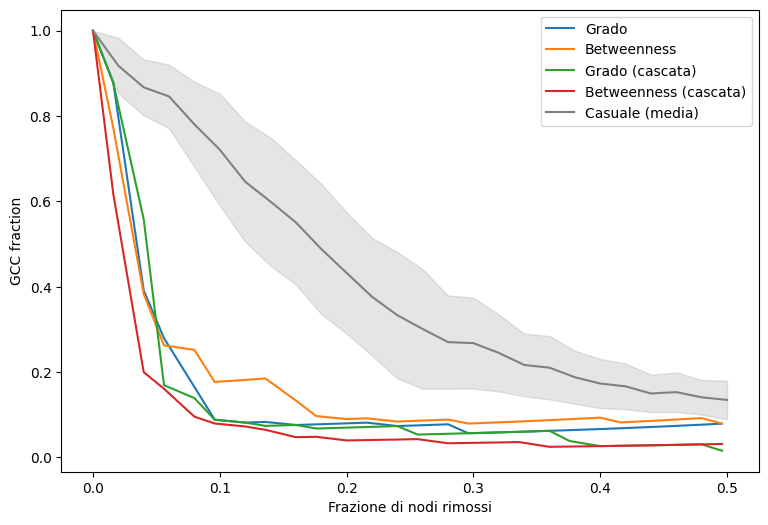
\includegraphics[width=0.8\linewidth]{Immagini//Capitoli//cap5/atk_cfr.png}
    \caption{Confronto attacchi di vulnerabilità}
    \label{fig: Confronto attacchi di vulnerabilità}
\end{figure}
\vspace{1em}

Operando il confronto, si conferma la decrescita \textbf{graduale} dell'attacco \textit{casuale}, rispetto alle altre tipologie di attacco che hanno una decrescita sensibilmente più \textbf{rapida}.

La rete metropolitana è quindi estremamente vulnerabile agli attacchi mirati su nodi con alto \textit{grado} o \textit{betweenness}, ma molto più robusta a f\textit{allimenti casuali}. Gli attacchi con effetto a cascata hanno l’impatto peggiore.

\vspace{1em}
\begin{figure}[h!]
    \centering
    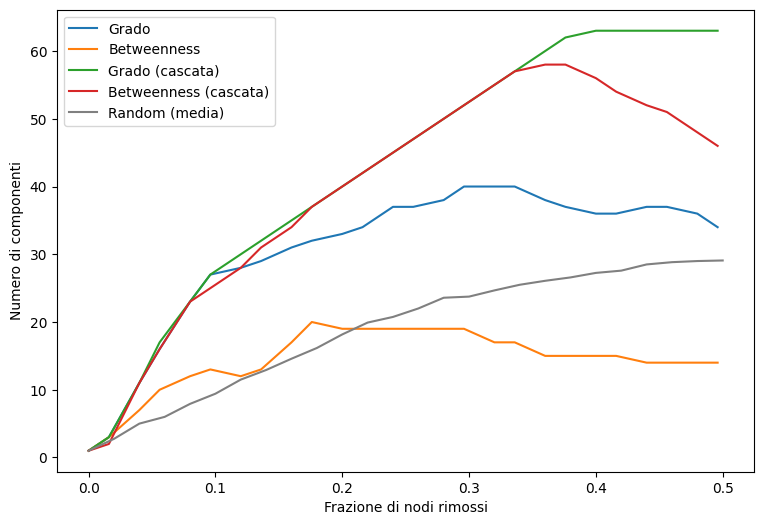
\includegraphics[width=0.8\linewidth]{Immagini//Capitoli//cap5/removed_cfr.png}
    \caption{Numero di componenti connesse in relazione alla rimozione di nodi}
    \label{fig: Numero di componenti connesse in relazione alla rimozione di nodi}
\end{figure}
\vspace{1em}

Un'altra analisi di confronto importante si può ritrovare in figura \ref{fig: Numero di componenti connesse in relazione alla rimozione di nodi}, in cui sono rappresentati il numero di componenti connessi nella rete che, partendo dall'unica iniziale, si degrada in più componenti connesse all'aumentare della frazione dei nodi rimossi.

Le curve degli attacchi a cascata crescono rapidamente e raggiungono oltre 60 componenti tra il 30\% e il 40\% di rimozione, la rete si frammenta \textbf{fortemente}.
La rimozione per grado mirata produce meno frammentazione, ma comunque notevole.

Una differenza rispetto alle analisi precedenti si ha nell'attacco per betweenness, che non produce un numero di componenti altrettanto alto, tende quindi a isolare nodi mantenendo gruppi più compatti.

L'attacco casuale aumenta più lentamente e si stabilizza tra i 25 e i 30 componenti, coerentemente con la maggiore robustezza casuale.

Le strategie basate su grado o betweenness in modalità a cascata frammentano quindi rapidamente la rete, evidenziando che la connettività globale dipende da pochi nodi centrali critici. Gli attacchi per betweenness mirati creano meno frammentazione rispetto agli altri attacchi mirati, ma comunque distruggono la connettività principale come evidenziato precedentemente.

Le aspettative derivanti dalle analisi svolte nei capitoli precedenti sono state quindi \textbf{confermate} dai risultati degli attacchi svolti.
\chapter{Conclusioni}

L’analisi condotta ha permesso di rappresentare e studiare la Rete di Trasporto Pubblica Metropolitana Milanese come una rete complessa, utilizzando un approccio di network analysis per descriverne le caratteristiche strutturali, topologiche e funzionali, e successivamente per valutarne la vulnerabilità a diverse tipologie di attacco.

A partire dai dataset ufficiali forniti dal Portale Open Data del Comune di Milano e da AMAT, si è costruita una rappresentazione a grafo accurata della rete, nella quale le fermate sono state modellate come nodi e i collegamenti diretti come archi. Tale modellazione in $\mathbb{L}$-Space ha consentito di ottenere una visione della struttura topologica della rete.

Le analisi descrittive hanno evidenziato come la PTN milanese presenti una configurazione prevalentemente lineare e radiale, con un grado medio vicino a 2 e un numero limitato di nodi maggiormente connessi. La rete risulta ben connessa e completamente unificata in un’unica componente connessa, con un’efficienza globale coerente con quella di infrastrutture geograficamente vincolate. Tuttavia, il coefficiente di clustering nullo e la disassortatività del grafo suggeriscono una rete ottimizzata per la distribuzione del traffico ma non particolarmente robusta a guasti localizzati.

L’analisi delle metriche di centralità ha permesso di individuare i nodi più rilevanti per la connettività complessiva: stazioni come Centrale FS, Cadorna, Garibaldi FS, Duomo e Loreto emergono come punti critici della rete, non solo per il loro grado ma anche per l’elevata betweenness e closeness, confermando il loro ruolo principale.

Lo studio di vulnerabilità ha infine messo in evidenza come la rete sia resiliente agli attacchi casuali, ma più sensibile ad attacchi mirati basati su misure di centralità. In particolare, la rimozione dei nodi più centrali comporta un rapido collasso della connettività: già con la rimozione del 10\% dei nodi principali, la Giant Connected Component si riduce drasticamente soprattutto negli scenari a cascata, che simulano in modo più realistico gli effetti di guasti successivi. 

Nel complesso, i risultati confermano che la Rete Metropolitana Milanese è progettata in modo efficiente per la mobilità quotidiana e garantisce buoni livelli di ridondanza nelle connessioni centrali. Tuttavia, la forte dipendenza da pochi nodi strategici la rende vulnerabile a interruzioni mirate.

\section{Sviluppi futuri}
In prospettiva, il modello sviluppato potrebbe essere esteso integrando dati dinamici per analizzare non solo la vulnerabilità strutturale ma anche quella funzionale, valutando l’impatto operativo di guasti o disservizi.



% ----------------------
% ---- BIBLIOGRAPHY ----
% ----------------------
\backmatter
\sloppy % serve a non far andare i link oltre ai margini
\printbibliography[heading=bibintoc, title=Bibliografia, ]


% ----------------------
% ---- DOCUMENT END ----
% ----------------------
\end{document} % Fine documento



